\documentclass[11pt,a4paper]{article}

% ----- Packages -----
\usepackage[margin=1in]{geometry}
\usepackage[utf8]{inputenc}
\usepackage[T1]{fontenc}
\usepackage{lmodern}
\usepackage{microtype}
\usepackage[dvipsnames,table]{xcolor}
\definecolor{BrandColor}{HTML}{3FADA8}
\usepackage{amsmath,amssymb}
\usepackage{titlesec}
\usepackage{tcolorbox}
\tcbuselibrary{skins,breakable,listings}
\usepackage{enumitem}
\usepackage{longtable,booktabs,array}
\usepackage{fancyhdr}
\usepackage[hidelinks,colorlinks=true,linkcolor=BrandColor,urlcolor=BrandColor,citecolor=BrandColor]{hyperref}
\usepackage[normalem]{ulem}
\usepackage{xurl}
\usepackage{graphicx}
\usepackage{float}
\usepackage{caption}
\usepackage{listings}
\usepackage{tabularx}
\usepackage{multirow}

% ----- Styling -----
\pagestyle{fancy}
\fancyhf{}
\fancyfootoffset[L,R]{0.75in}
\setlength{\headheight}{32pt}
\addtolength{\topmargin}{-16pt}
\renewcommand{\headrulewidth}{0.5pt}
\renewcommand{\footrulewidth}{0.5pt}

\fancyhead[L]{\textsf{\textbf{CSE638: Graduate Systems (GRS)}}\\\textsf{\textbf{Winter 2026}}}
\fancyhead[R]{\textsf{\textbf{P1: Kubernetes CNI Plugins}}\\\textsf{\textbf{Comprehensive Report}}}
\fancyfoot[C]{\footnotesize\textsf{\thepage}}

\titleformat{\section}
  {\normalfont\Large\sffamily\bfseries\color{BrandColor}}
  {\thesection.}{0.5em}{}[{\vspace{0.1cm}\color{BrandColor}\titlerule[0.3pt]}]

\titleformat{\subsection}
  {\normalfont\large\sffamily\bfseries\color{BrandColor!80!black}}
  {\thesubsection}{0.5em}{}

\titleformat{\subsubsection}
  {\normalfont\normalsize\sffamily\bfseries\color{BrandColor!60!black}}
  {\thesubsubsection}{0.5em}{}

\titleformat{\paragraph}[runin]
  {\normalfont\normalsize\sffamily\bfseries\color{BrandColor!60!black}}
  {}{0em}{}

\lstset{
  basicstyle=\ttfamily\small,
  backgroundcolor=\color{gray!5},
  frame=single,
  rulecolor=\color{gray!30},
  breaklines=true,
  tabsize=2,
  showstringspaces=false,
}

\newtcolorbox{infobox}[1][]{
  enhanced, colback=BrandColor!5, colframe=BrandColor!70,
  fonttitle=\bfseries\sffamily, title=#1, breakable
}

\newtcolorbox{resultbox}[1][]{
  enhanced, colback=green!3, colframe=green!50!black,
  fonttitle=\bfseries\sffamily, title=#1, breakable
}

\newtcolorbox{findingbox}[1][]{
  enhanced, colback=orange!5, colframe=orange!70!black,
  fonttitle=\bfseries\sffamily, title=#1, breakable
}

% ----- Document -----
\begin{document}

% ======================== TITLE PAGE ========================
\begin{titlepage}
\thispagestyle{empty}
\begin{center}
\vspace*{0.5cm}


\includegraphics[width=4cm]{1_iiitd_logo.png}\\[1cm]

{\LARGE\textsf{\textbf{Indraprastha Institute of Information Technology, Delhi}}}\\[0.5cm]
{\large\textsf{CSE638: Graduate Systems (GRS) --- Winter 2026}}\\[0.3cm]
{\large\textsf{Instructor: Dr.\ Rinku Shah}}\\[1.5cm]

\rule{\textwidth}{0.5pt}\\[0.8cm]
{\Huge\textsf{\textbf{\textcolor{BrandColor}{Performance Comparison of\\[0.3cm]Kubernetes CNI Plugins}}}}\\[0.8cm]
\rule{\textwidth}{0.5pt}\\[1cm]

{\Large\textsf{\textbf{Comprehensive Report: Kind Cluster \& Bare-Metal Cluster}}}\\[1.5cm]

{\large\textsf{\textbf{Group 1}}}\\[0.3cm]
\begin{tabular}{ll}
  Yash Kumar Vaibhav & MT25091 \\
  Nishit Jain & MT25004 \\
  Prakhar Agarwal & MT25005 \\
  Reehan Sarmah & MT25036 \\
  Samyak Kr.\ Sharma & MT25039 \\
\end{tabular}\\[1.5cm]

{\large\textsf{GitHub: \url{https://github.com/yashkumarvaibhav/GrS-CSE638_Project}}}\\[0.5cm]
{\large\textsf{\today}}

\end{center}
\end{titlepage}

% ======================== TABLE OF CONTENTS ========================
\newpage
\tableofcontents
\newpage

% ======================== 1. ABSTRACT ========================
\section{Abstract}

This report presents a comprehensive performance comparison of three Kubernetes Container Network Interface (CNI) plugins---\textbf{Flannel}, \textbf{Calico}, and \textbf{Cilium}---across two fundamentally different deployment environments:
\begin{itemize}[nosep]
  \item \textbf{Part~A --- Kind Cluster (Intra-Node):} A \texttt{kind} cluster on a 128-core AMD EPYC server, evaluating same-node, cross-node, and ClusterIP Service topologies across three payload sizes (64\,B, 4\,KB, 1\,MB), three concurrency levels (1, 16, 64), and three extension experiments (NetworkPolicy, WireGuard, kube-proxy replacement).
  \item \textbf{Part~B --- Bare-Metal Cluster (Multi-Node):} A 3-node Kubernetes cluster on physical laptops connected over WiFi, comparing six CNI configurations (3 CNIs $\times$ 2 routing modes: VXLAN overlay vs.\ underlay routing) across TCP throughput, TCP\_RR latency, HTTP latency, UDP performance, and CPU/memory overhead.
\end{itemize}

\noindent\textbf{Kind-cluster key findings:} Cilium achieves the highest throughput (up to 63.98\,Gbps same-node) via its eBPF datapath, while Flannel delivers the lowest latency (24.18\,$\mu$s cross-node TCP\_RR). WireGuard encryption imposes severe overhead ($+537\%$ latency for Calico, $+365\%$ for Cilium). NetworkPolicy shows divergent effects: $-45\%$ throughput for Calico but $+118\%$ for Cilium (high CV; interpret with caution).

\noindent\textbf{Bare-metal key findings:} Calico VXLAN and Flannel VXLAN lead TCP throughput ($\approx$0.119\,Gbps), while Cilium VXLAN is unexpectedly slowest (0.058\,Gbps) yet delivers the best HTTP latency (P50\,=\,6.56\,ms). For UDP, Calico BGP leads (11.88\,Mbps, 38\% loss) while Calico VXLAN degrades severely (5.78\,Mbps, 68\% loss). CPU overhead is modest across all CNIs (3.9--6.0\% node-level).

\noindent\textbf{Cross-environment insight:} CNI performance rankings shift dramatically between environments. Cilium leads throughput in kind-cluster but trails in bare-metal WiFi, demonstrating that CNI selection must be validated on representative hardware. The physical network medium---not the CNI---emerges as the dominant bottleneck on constrained networks, compressing all CNIs into a narrow throughput band.

% ======================== 2. INTRODUCTION ========================
\section{Introduction}

\subsection{Problem}

Kubernetes relies on CNI plugins to provide pod-to-pod and pod-to-service networking. The choice of CNI directly impacts application performance, latency-sensitive microservice communication, and operational costs. While vendor-provided benchmarks and blog posts exist, few provide systematic, reproducible comparisons using consistent methodology across different deployment environments.

\subsection{Motivation}

Production Kubernetes clusters span a wide spectrum of hardware---from intra-node development environments to multi-node bare-metal clusters with real network interconnects. Understanding how CNI plugins perform across this spectrum is critical because:
\begin{itemize}
  \item Performance characteristics observed in simulated environments (kind, minikube) may not transfer to production hardware.
  \item Architectural decisions like overlay vs.\ underlay routing have environment-dependent trade-offs.
\end{itemize}

This study bridges the gap by benchmarking the same three CNIs in both a kind-cluster (intra-node) and a bare-metal (multi-node WiFi) environment, enabling direct cross-environment comparison.

\subsection{Objectives}
\begin{enumerate}
  \item Compare TCP/UDP throughput, latency, and HTTP performance across all three CNIs
  \item Evaluate overlay (VXLAN) vs.\ underlay routing modes for each CNI on bare-metal hardware.
  \item Measure CPU overhead at node granularity.
  \item Analyze how deployment environment affects CNI performance rankings
\end{enumerate}

% ======================== 3. BACKGROUND ========================
\section{Background}

\subsection{Kubernetes Networking Model}

Kubernetes mandates a flat network where every pod receives a unique IP address and can communicate with every other pod without NAT. The Container Network Interface (CNI) specification defines how plugins attach network interfaces to containers. When a pod is created, the kubelet invokes the configured CNI plugin to assign an IP, configure routes, and potentially establish overlay tunnels between nodes.

\subsection{Overlay vs.\ Underlay Routing}

\begin{itemize}
  \item \textbf{Overlay (VXLAN):} Pod packets are encapsulated in UDP headers (VXLAN, Virtual Extensible LAN) before traversing the physical network. Adds 50 bytes overhead per packet but works across any IP-reachable infrastructure.
  \item \textbf{Underlay routing:} Pod subnets are advertised directly to the host network. Mechanism varies per CNI:
  \begin{itemize}
    \item \textbf{Flannel Host-GW:} Static routes on each node. Requires L2 adjacency.
    \item \textbf{Calico BGP:} BGP daemon (BIRD) exchanges pod subnet routes. Works across L3 boundaries.
    \item \textbf{Cilium Underlay Routing:} Linux kernel routing with eBPF packet steering. Requires L2 adjacency.
  \end{itemize}
  \item \textbf{eBPF-based datapaths:} Attach BPF programs to kernel hooks (TC/XDP) to short-circuit the traditional networking stack. Reduces per-packet overhead at the cost of implementation complexity.
\end{itemize}

\subsection{CNI Plugins Under Test}

\begin{itemize}[leftmargin=2cm]
  \item[\textcolor{BrandColor}{\textbf{Flannel}}] Lightweight CNI supporting VXLAN overlay and Host-GW underlay routing. No native NetworkPolicy support. Simplest architecture with minimal resource footprint.
  \item[\textcolor{red!70!black}{\textbf{Calico}}] Feature-rich CNI supporting VXLAN overlay, BGP-based underlay routing, and IPinIP encapsulation. Full NetworkPolicy enforcement via iptables.
  \item[\textcolor{cyan!60!black}{\textbf{Cilium}}] eBPF-based CNI supporting VXLAN overlay and underlay routing. Attaches eBPF programs to TC/XDP hooks for fast-path processing. 
\end{itemize}


% ========================================================================
% PART A: KIND CLUSTER
% ========================================================================
\newpage
\section{Part A: Kind Cluster (Intra-Node) Benchmarking}

\subsection{Methodology}

\subsubsection{Test Environment}

\begin{infobox}[Hardware \& Software Specifications]
\begin{tabularx}{\textwidth}{lX}
  \toprule
  \textbf{Component} & \textbf{Details} \\
  \midrule
  CPU & AMD EPYC 7713 (128 cores / 256 threads) \\
  RAM & 125\,GB DDR4 \\
  Disk & 833\,GB available \\
  OS & Ubuntu 22.04 LTS (kernel 5.15.0-71) \\
  Container Runtime & Docker 26.1.3 \\
  Kubernetes & kind v0.25.0 (K8s v1.31) \\
  \bottomrule
\end{tabularx}
\end{infobox}

Each CNI is deployed on a 3-node kind cluster (1 control-plane, 2 workers) with \texttt{disableDefaultCNI: true}. Pod CIDR: \texttt{10.244.0.0/16}. kube-proxy is retained in all baseline configurations for fair comparison. CNI versions: Flannel v0.26.1, Calico v3.29.1, Cilium v1.16.5.

\subsubsection{Test Scenarios}

\begin{longtable}{p{1.5cm}p{4cm}p{3cm}p{5cm}}
  \toprule
  \textbf{ID} & \textbf{Description} & \textbf{Nodes} & \textbf{Target} \\
  \midrule
  T1 & Same-node pod-to-pod & worker $\to$ worker & Direct Pod IP \\
  T2 & Cross-node pod-to-pod & worker $\to$ worker2 & Direct Pod IP \\
  T3 & Cross-node via Service & worker $\to$ worker2 & ClusterIP Service \\
  \bottomrule
\end{longtable}

\subsubsection{Test Matrix}

\begin{itemize}[nosep]
  \item \textbf{Payload sizes:} 64\,B, 4\,KB, 1\,MB
  \item \textbf{Concurrency levels:} 1, 16, 64 parallel streams
  \item \textbf{Repetitions:} 3 per configuration
  \item \textbf{Duration:} 10\,s per test
  \item Total: $3 \times 3 \times 3 \times 3 = 81$ baseline tests per CNI per tool (729 total)
\end{itemize}

\subsubsection{Benchmark Tools}

\begin{longtable}{p{2cm}p{3cm}p{8cm}}
  \toprule
  \textbf{Tool} & \textbf{Version} & \textbf{Metrics Collected} \\
  \midrule
  iperf3 & digest-pinned & TCP throughput (Gbps), UDP throughput, jitter, loss \\
  netperf & digest-pinned & TCP\_RR transaction rate (/s), mean latency ($\mu$s) \\
  fortio & digest-pinned & HTTP QPS, percentile latencies (p50, p90, p99) \\
  docker stats & --- & CPU \%, memory usage per container \\
  \bottomrule
\end{longtable}

\subsubsection{Extension Experiments}

\begin{longtable}{p{1.5cm}p{3cm}p{3cm}p{5.5cm}}
  \toprule
  \textbf{ID} & \textbf{Extension} & \textbf{CNIs} & \textbf{Configuration} \\
  \midrule
  E1 & NetworkPolicy & Calico, Cilium & allow-all policy applied \\
  E2 & WireGuard & Calico, Cilium & Node-to-node encryption \\
  E3 & KPR mode & Cilium only & \texttt{kubeProxyReplacement=true} \\
  \bottomrule
\end{longtable}

Extension tests use 4\,KB payload, concurrency 16, and 5 repetitions.

\subsection{Implementation}

\subsubsection{Cluster Setup}

Each CNI was tested on a dedicated \texttt{kind} cluster created by \texttt{scripts/1\_setup\_cluster.sh}.
The script provisions a 3-node cluster (1 control-plane, 2 workers), disables the default CNI,
copies the CNI plugins tarball (\texttt{cni-plugins-linux-amd64-v1.9.0.tgz}) to each node via \texttt{docker cp},
and then installs the requested CNI using Helm (Calico via Tigera operator, Cilium via Cilium chart) or
\texttt{kubectl apply} (Flannel).
For the Cilium KPR experiment (E3), the script additionally deletes the \texttt{kube-proxy} DaemonSet and ConfigMap
before installing Cilium with \texttt{kubeProxyReplacement=true}.

\subsubsection{Benchmark Automation}

All data collection is performed by a single canonical script, \texttt{scripts/1\_fast\_benchmark.py} ($\approx$390 lines of Python).
The script:
\begin{enumerate}
  \item Deploys server and client pods on designated nodes using topology-appropriate \texttt{nodeSelector} labels.
  \item Iterates over each (topology, payload, concurrency, repetition) combination.
  \item For each combination, invokes \texttt{kubectl exec} to run the benchmark tool (iperf3, netperf, or fortio) inside the client pod.
  \item Parses stdout to extract the primary metric: iperf3 and fortio use JSON output parsing; netperf uses reversed-line token extraction from its text-format output.
  \item Collects \texttt{docker stats} samples via best-effort periodic polling (approximately every 3\,s in practice) during each benchmark window to record CPU and memory usage of kind node containers.
  \item Appends results to per-tool CSV files with columns for topology, message size, concurrency, repetition, and the measured value.
\end{enumerate}

\subsubsection{Data Processing and Visualization}

After collection, \texttt{scripts/1\_aggregate\_data.py} computes per-configuration mean and standard deviation across repetitions and exports the results as JSON.
Ten plot scripts in \texttt{plots/} generate publication-quality figures from hardcoded aggregated values.
The report is typeset with Tectonic/\LaTeX.

\subsection{Evaluation and Observations}

\subsubsection{TCP Throughput (iperf3)}

\begin{figure}[H]
  \centering
  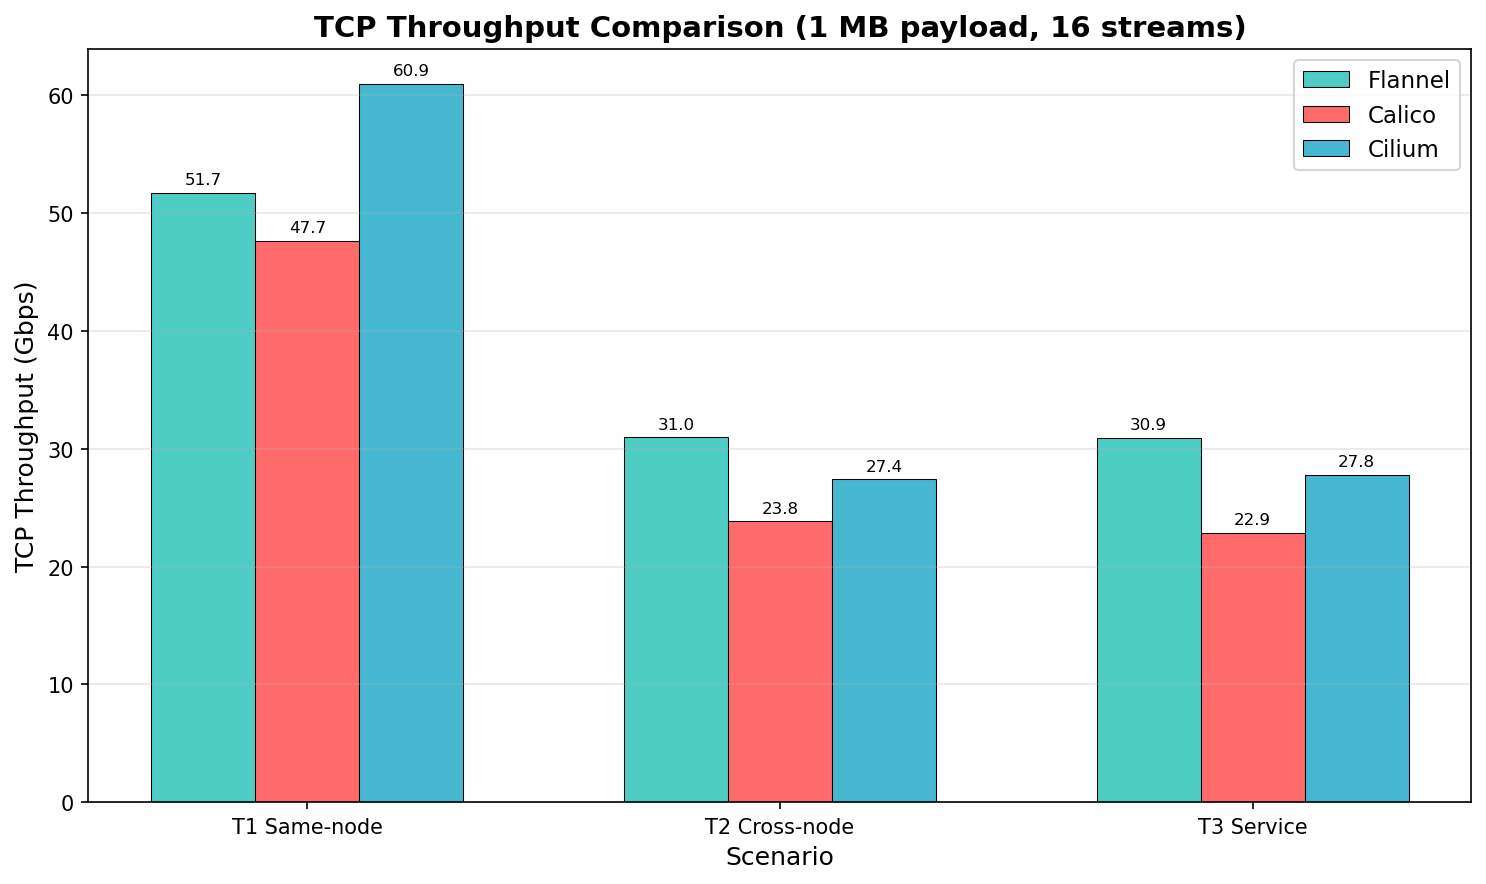
\includegraphics[width=\textwidth]{kind-cluster/plots/1_throughput_comparison.png}
  \caption{TCP throughput comparison across CNI plugins and scenarios (1\,MB payload, 16 streams).}
  \label{fig:kc-throughput}
\end{figure}

\begin{table}[H]
\centering
\caption{T1 Same-Node TCP Throughput (Gbps) --- Mean over 3 reps}
\begin{tabular}{llrrr}
  \toprule
  \textbf{Size} & \textbf{Concurrency} & \textbf{Flannel} & \textbf{Calico} & \textbf{Cilium} \\
  \midrule
  64\,B  & 1  & 0.46 & 0.44 & 0.43 \\
  64\,B  & 16 & 0.79 & 0.54 & 0.62 \\
  64\,B  & 64 & 0.68 & 0.56 & 0.67 \\
  4\,KB  & 1  & 5.26 & 3.65 & 5.50 \\
  4\,KB  & 16 & 4.75 & 6.53 & 8.32 \\
  4\,KB  & 64 & 4.78 & 3.45 & 5.65 \\
  1\,MB  & 1  & 60.93 & 49.61 & 63.98 \\
  1\,MB  & 16 & 51.72 & 47.67 & 60.94 \\
  1\,MB  & 64 & 36.04 & 34.43 & 39.33 \\
  \bottomrule
\end{tabular}
\label{tab:kc-t1}
\end{table}

\begin{table}[H]
\centering
\caption{T2 Cross-Node TCP Throughput (Gbps) --- Mean over 3 reps}
\begin{tabular}{llrrr}
  \toprule
  \textbf{Size} & \textbf{Concurrency} & \textbf{Flannel} & \textbf{Calico} & \textbf{Cilium} \\
  \midrule
  64\,B  & 1  & 0.46 & 0.29 & 0.44 \\
  64\,B  & 16 & 0.61 & 0.53 & 0.55 \\
  64\,B  & 64 & 0.47 & 0.41 & 0.45 \\
  4\,KB  & 1  & 1.94 & 1.35 & 3.27 \\
  4\,KB  & 16 & 1.88 & 6.30 & 2.32 \\
  4\,KB  & 64 & 1.82 & 1.27 & 1.66 \\
  1\,MB  & 1  & 32.97 & 24.01 & 29.92 \\
  1\,MB  & 16 & 30.96 & 23.83 & 27.40 \\
  1\,MB  & 64 & 27.69 & 19.97 & 25.78 \\
  \bottomrule
\end{tabular}
\label{tab:kc-t2}
\end{table}

\begin{table}[H]
\centering
\caption{T3 ClusterIP Service TCP Throughput (Gbps) --- Mean over 3 reps}
\begin{tabular}{llrrr}
  \toprule
  \textbf{Size} & \textbf{Concurrency} & \textbf{Flannel} & \textbf{Calico} & \textbf{Cilium} \\
  \midrule
  64\,B  & 1  & 0.47 & 0.29 & 0.43 \\
  64\,B  & 16 & 0.60 & 0.54 & 0.53 \\
  64\,B  & 64 & 0.46 & 0.40 & 0.45 \\
  4\,KB  & 1  & 1.90 & 1.38 & 2.98 \\
  4\,KB  & 16 & 1.82 & 3.30 & 5.85 \\
  4\,KB  & 64 & 1.81 & 1.26 & 1.64 \\
  1\,MB  & 1  & 34.13 & 24.11 & 32.42 \\
  1\,MB  & 16 & 30.92 & 22.87 & 27.78 \\
  1\,MB  & 64 & 27.00 & 20.11 & 25.05 \\
  \bottomrule
\end{tabular}
\label{tab:kc-t3}
\end{table}

\begin{findingbox}[Kind-Cluster Throughput Key Observations]
\begin{enumerate}
  \item \textbf{Cilium leads in throughput}: 63.98\,Gbps same-node (1\,MB/$c{=}1$), benefiting from eBPF fast-path that bypasses portions of the kernel networking stack. At 4\,KB/$c{=}16$, Cilium reaches 8.32\,Gbps---75\% higher than Flannel's 4.75\,Gbps.
  \item \textbf{VXLAN encapsulation cost}: Cross-node (T2) throughput is $40{-}60\%$ lower than same-node (T1) due to overlay processing. Service (T3) adds $0{-}10\%$ additional overhead from kube-proxy's iptables DNAT.
  \item \textbf{Calico trails in raw performance}: 49.61\,Gbps same-node vs.\ Cilium's 63.98\,Gbps, attributable to iptables-based packet processing overhead.
  \item \textbf{Calico anomalous spike}: 6.30\,Gbps at T2/4\,KB/$c{=}16$, likely due to aggressive TCP segmentation offload under specific buffer conditions.
\end{enumerate}
\end{findingbox}

\subsubsection{Latency (netperf TCP\_RR)}

\begin{figure}[H]
  \centering
  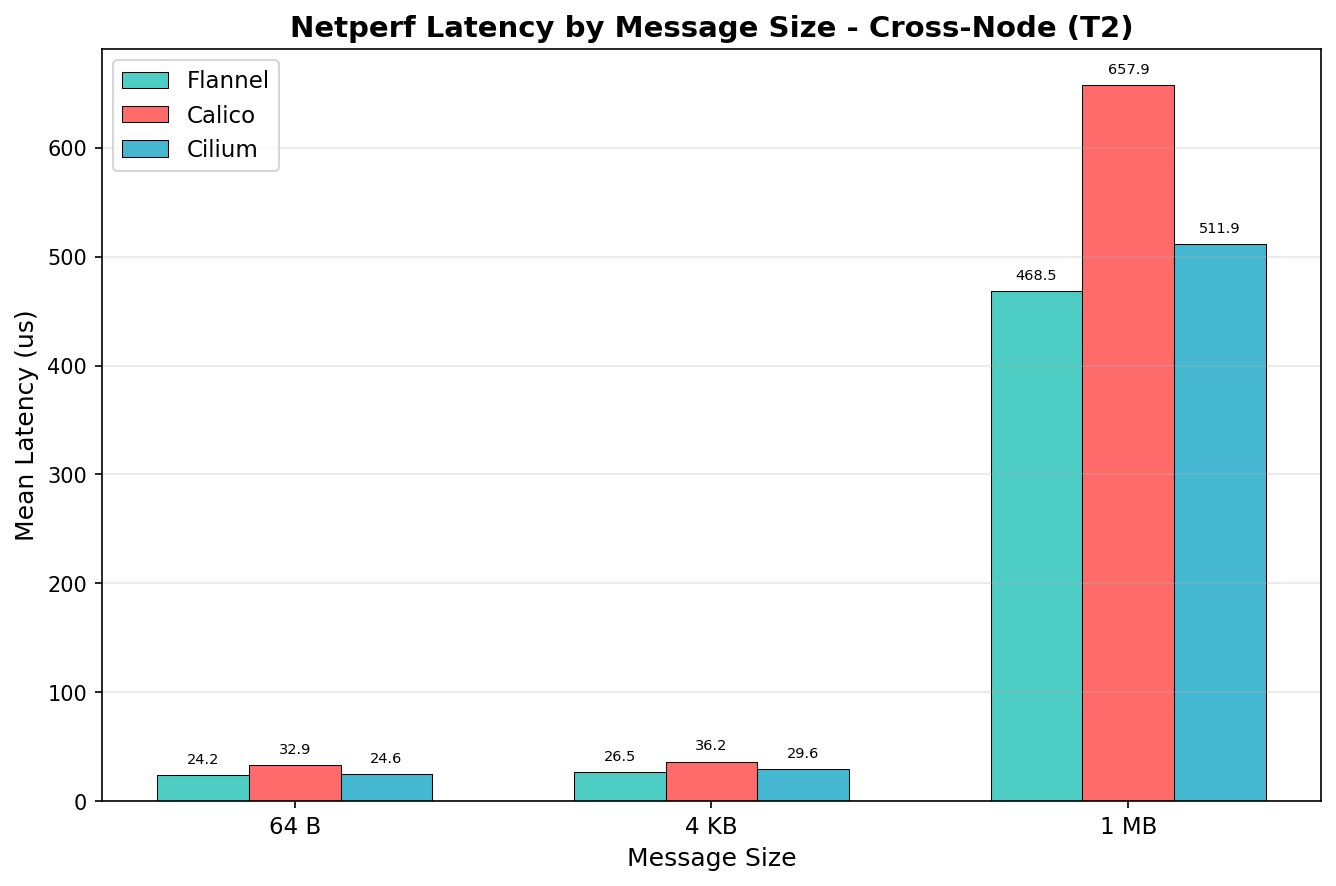
\includegraphics[width=\textwidth]{kind-cluster/plots/1_latency_comparison.png}
  \caption{Netperf TCP\_RR mean latency by message size (T2 cross-node, $c{=}1$).}
  \label{fig:kc-latency}
\end{figure}

\begin{table}[H]
\centering
\caption{TCP\_RR Transaction Rate (trans/s) and Mean Latency ($\mu$s) --- T2, $c=1$}
\begin{tabular}{lrrrrrr}
  \toprule
  \multirow{2}{*}{\textbf{Size}} & \multicolumn{2}{c}{\textbf{Flannel}} & \multicolumn{2}{c}{\textbf{Calico}} & \multicolumn{2}{c}{\textbf{Cilium}} \\
  \cmidrule(lr){2-3}\cmidrule(lr){4-5}\cmidrule(lr){6-7}
  & Trans/s & $\mu$s & Trans/s & $\mu$s & Trans/s & $\mu$s \\
  \midrule
  64\,B  & 41{,}350 & 24.18 & 30{,}391 & 32.91 & 40{,}600 & 24.63 \\
  4\,KB  & 37{,}733 & 26.51 & 27{,}589 & 36.25 & 33{,}822 & 29.57 \\
  1\,MB  & 2{,}135 & 468.48 & 1{,}520 & 657.85 & 1{,}954 & 511.91 \\
  \bottomrule
\end{tabular}
\label{tab:kc-latency}
\end{table}

\begin{findingbox}[Kind-Cluster Latency Key Observations]
\begin{enumerate}
  \item \textbf{Flannel delivers lowest latency}: 24.18\,$\mu$s for 64\,B TCP\_RR, closely followed by Cilium at 24.63\,$\mu$s. Calico is 36\% slower at 32.91\,$\mu$s due to iptables traversal.
  \item \textbf{Large payloads dominate}: At 1\,MB, all CNIs show dramatically higher latencies (468--658\,$\mu$s), reflecting serialization delay rather than CNI overhead.
  \item \textbf{Latency stable across concurrency}: TCP\_RR single-flow is not contention-bound in this intra-node environment.
\end{enumerate}
\end{findingbox}

\noindent\textit{Note:} Netperf through T3 (ClusterIP Service) returned zero for both TCP\_RR and TCP\_STREAM across all CNIs---a limitation of running netperf through kube-proxy's iptables DNAT, which disrupts the control connection. T3 netperf data is excluded from analysis.

\subsubsection{HTTP Performance (Fortio)}

\begin{figure}[H]
  \centering
  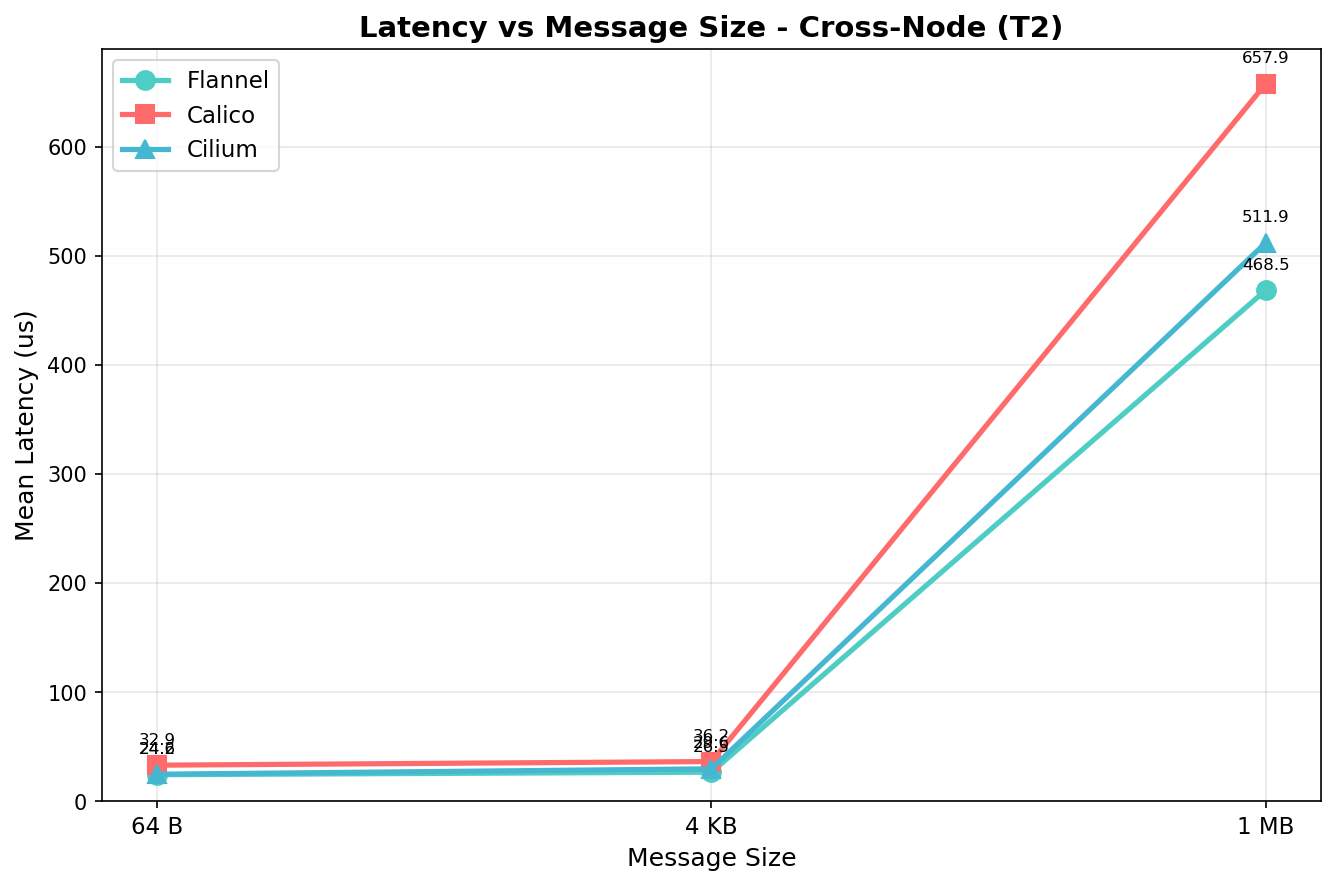
\includegraphics[width=\textwidth]{kind-cluster/plots/1_latency_vs_msgsize.png}
  \caption{Netperf mean latency vs.\ payload size across CNI plugins (T2 cross-node, $c{=}1$).}
  \label{fig:kc-latency-msgsize}
\end{figure}

\begin{table}[H]
\centering
\caption{Fortio HTTP QPS --- T2 Cross-Node, Mean over 3 reps}
\begin{tabular}{llrrr}
  \toprule
  \textbf{Size} & \textbf{Concurrency} & \textbf{Flannel} & \textbf{Calico} & \textbf{Cilium} \\
  \midrule
  64\,B  & 1  & 7{,}601 & 6{,}583 & 7{,}870 \\
  64\,B  & 16 & 81{,}749 & 74{,}792 & 132{,}836 \\
  64\,B  & 64 & 109{,}336 & 115{,}000 & 115{,}234 \\
  4\,KB  & 1  & 5{,}069 & 4{,}195 & 4{,}650 \\
  4\,KB  & 16 & 30{,}953 & 29{,}147 & 49{,}816 \\
  4\,KB  & 64 & 53{,}045 & 57{,}330 & 60{,}647 \\
  1\,MB  & 1  & 798 & 694 & 770 \\
  1\,MB  & 16 & 3{,}754 & 4{,}195 & 4{,}037 \\
  1\,MB  & 64 & 3{,}884 & 4{,}419 & 4{,}131 \\
  \bottomrule
\end{tabular}
\label{tab:kc-fortio}
\end{table}

\subsubsection{Throughput Scaling with Concurrency}

\begin{figure}[H]
  \centering
  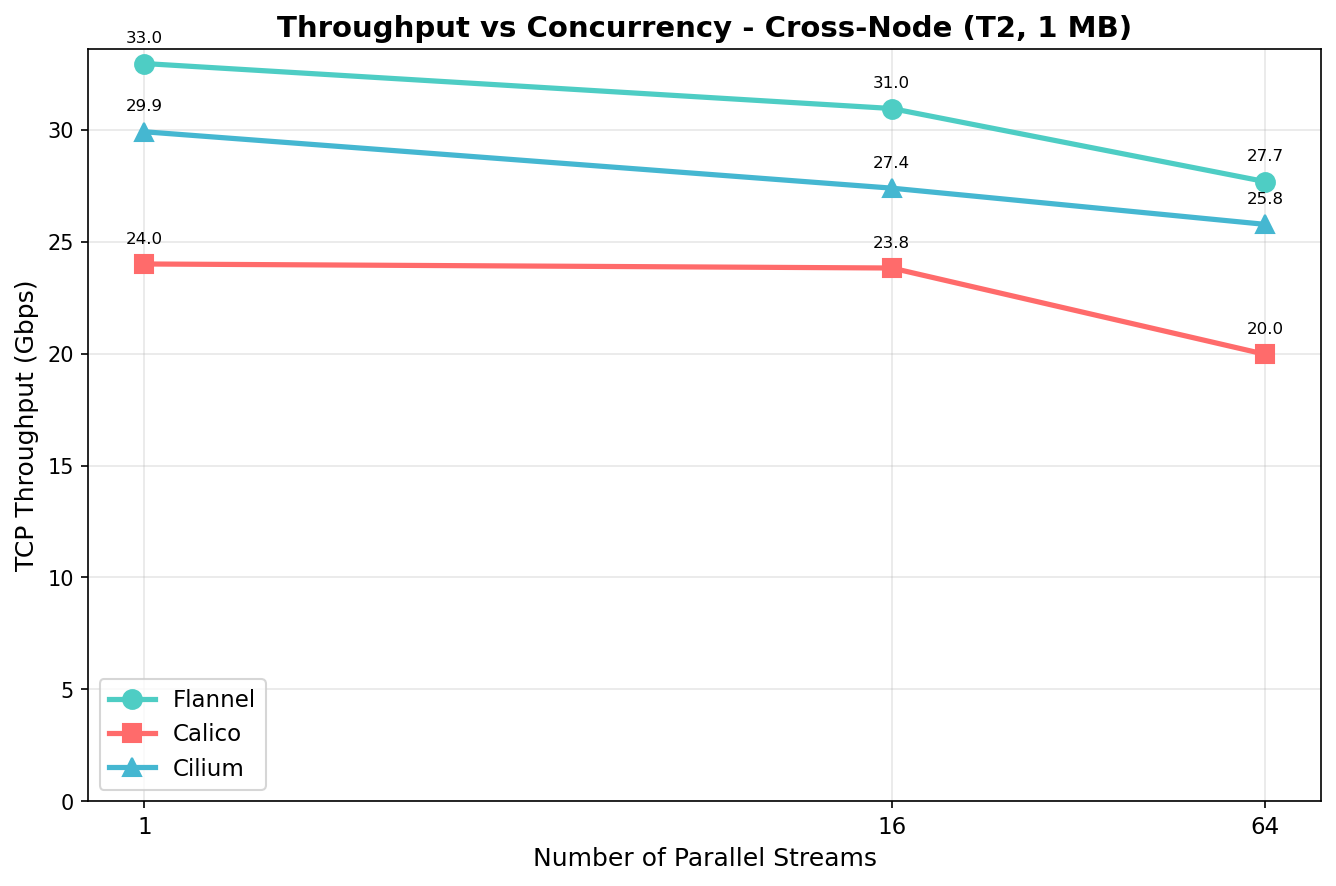
\includegraphics[width=\textwidth]{kind-cluster/plots/1_throughput_vs_concurrency.png}
  \caption{TCP throughput scaling with concurrent streams (T2 cross-node, 1\,MB payload).}
  \label{fig:kc-concurrency}
\end{figure}

\subsubsection{Pod Startup Time}

\begin{figure}[H]
  \centering
  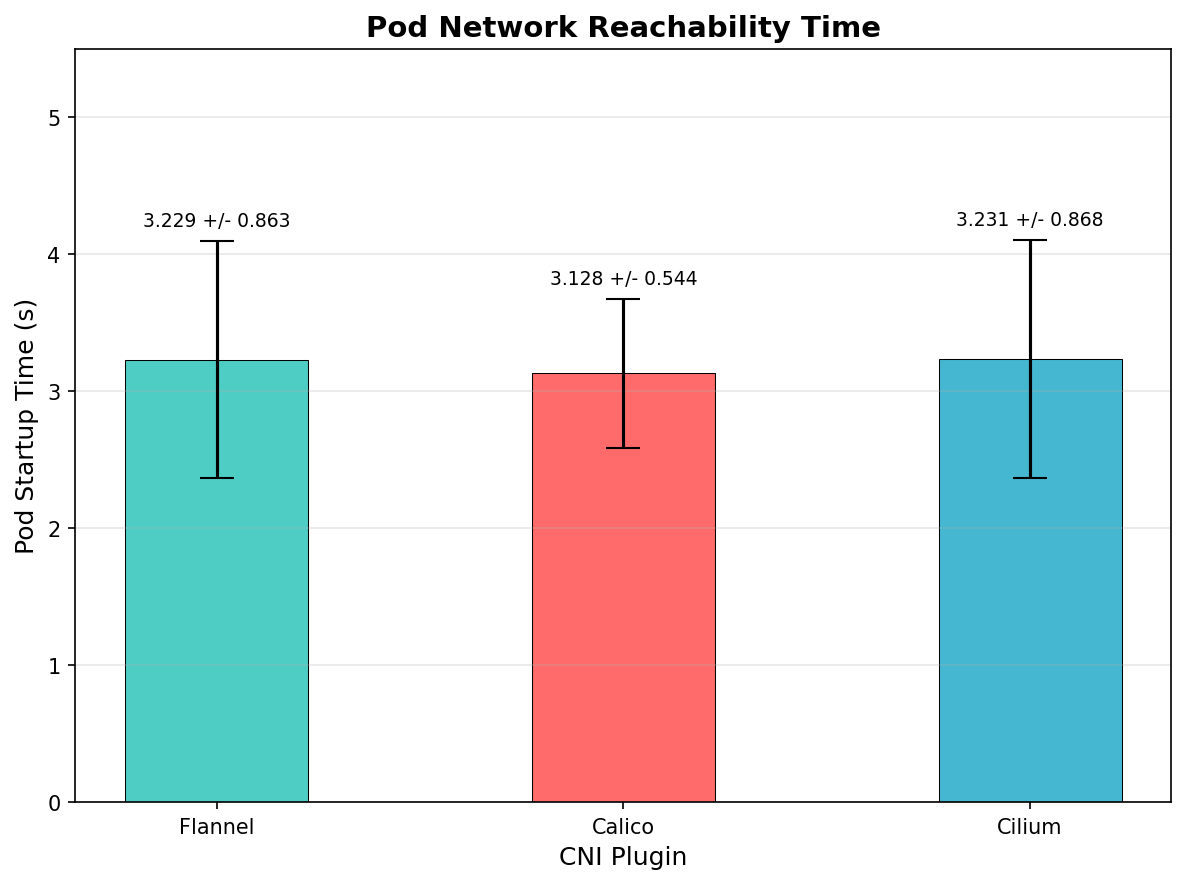
\includegraphics[width=0.7\textwidth]{kind-cluster/plots/1_pod_startup_time.png}
  \caption{Pod network reachability time across CNI plugins.}
  \label{fig:kc-startup}
\end{figure}

\begin{table}[H]
\centering
\caption{Pod Network Reachability Time (seconds) --- 10 iterations}
\begin{tabular}{lrrr}
  \toprule
  \textbf{Metric} & \textbf{Flannel} & \textbf{Calico} & \textbf{Cilium} \\
  \midrule
  Mean   & 3.229 & 3.128 & 3.231 \\
  Stdev  & 0.863 & 0.544 & 0.868 \\
  Min    & 2.945 & 2.952 & 2.952 \\
  Max    & 5.686 & 4.680 & 5.701 \\
  \bottomrule
\end{tabular}
\label{tab:kc-startup}
\end{table}

\subsubsection{Resource Overhead}

\begin{figure}[H]
  \centering
  \begin{minipage}{0.48\textwidth}
    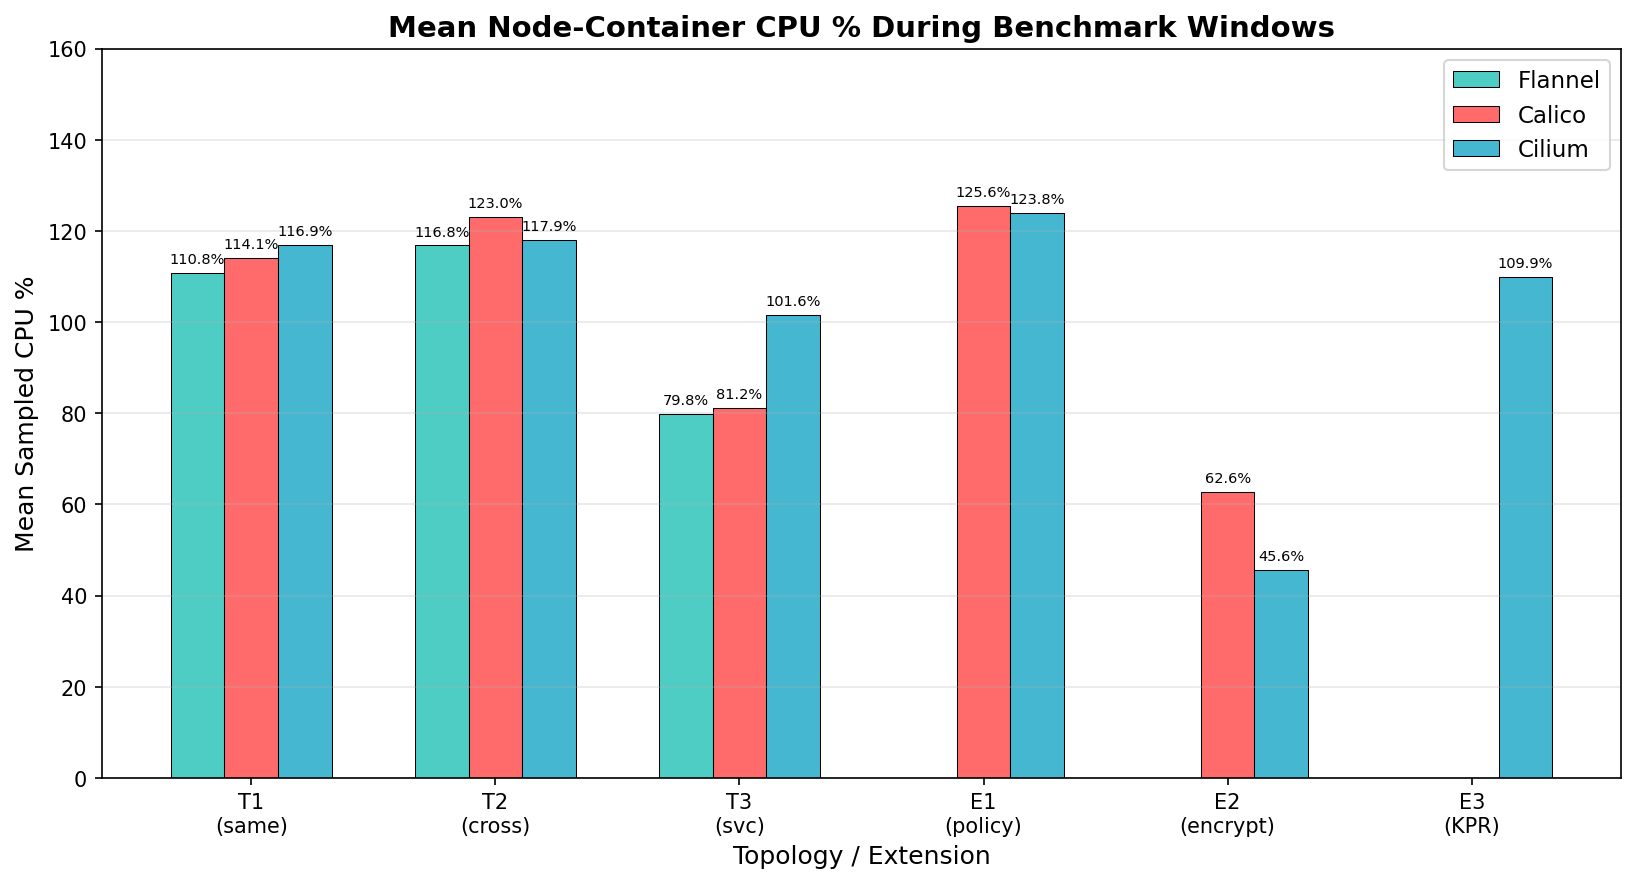
\includegraphics[width=\textwidth]{kind-cluster/plots/1_cpu_overhead.png}
    \caption{Mean sampled node-container CPU\,\% during benchmark windows.}
    \label{fig:kc-cpu}
  \end{minipage}\hfill
  \begin{minipage}{0.48\textwidth}
    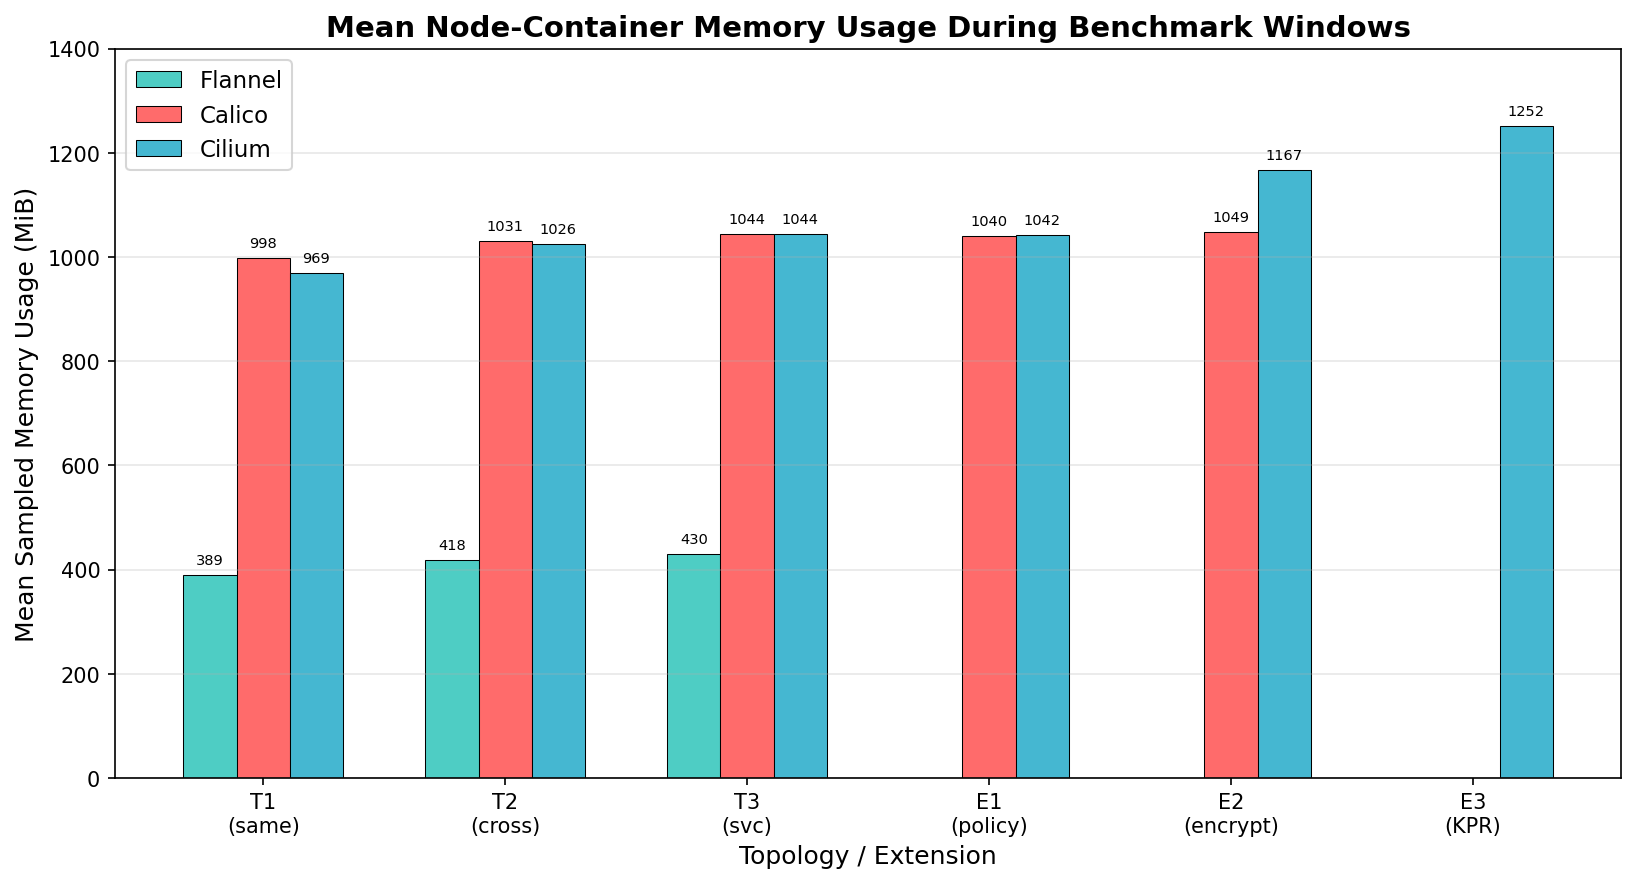
\includegraphics[width=\textwidth]{kind-cluster/plots/1_memory_overhead.png}
    \caption{Mean sampled node-container memory usage (MiB) during benchmark windows.}
    \label{fig:kc-memory}
  \end{minipage}
\end{figure}

Docker stats were collected via best-effort periodic sampling (approximately every 3\,s in practice) during each benchmark window to characterize node-container resource usage. Flannel nodes averaged 389--430\,MiB memory across topologies, while Calico (998--1049\,MiB) and Cilium (969--1044\,MiB) consumed $2.4{-}2.6\times$ more due to their richer control planes. Mean CPU\,\% was comparable at 101--117\% across CNIs for baseline topologies. WireGuard encryption (E2) markedly reduced CPU utilization---Calico dropped to 63\% and Cilium to 46\%---because encrypted sessions throttle aggregate throughput, leaving CPU idle. Cilium KPR (E3) had negligible resource impact (110\% CPU, 1252\,MiB memory) relative to baseline.

\subsection{Extension Experiments}

\subsubsection{E1: NetworkPolicy Enforcement Overhead}

\begin{figure}[H]
  \centering
  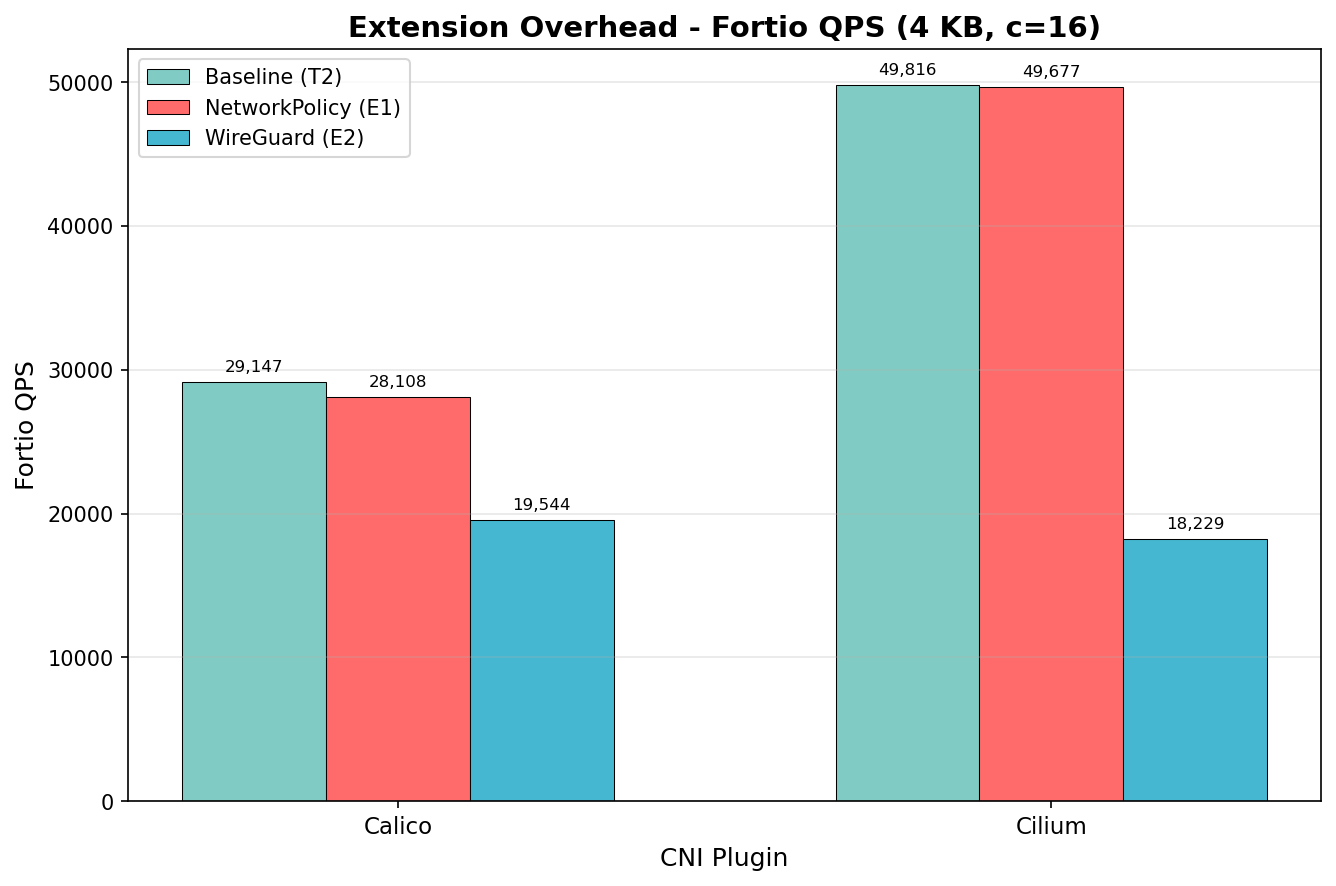
\includegraphics[width=0.8\textwidth]{kind-cluster/plots/1_network_policy_overhead.png}
  \caption{Extension overhead on Fortio QPS: baseline vs.\ E1 (NetworkPolicy) vs.\ E2 (WireGuard), 4\,KB, $c{=}16$.}
  \label{fig:kc-netpol}
\end{figure}

\begin{findingbox}[E1 Key Finding]
NetworkPolicy enforcement with an ``allow-all'' policy shows divergent effects across CNIs. For \textbf{Calico}, TCP throughput drops from 6.30\,Gbps to 3.44\,Gbps ($-45\%$), while latency and transaction rates remain virtually unchanged (36.18 vs.\ 36.28\,$\mu$s). Fortio QPS decreases marginally from 29{,}147 to 28{,}108 ($-3.6\%$). For \textbf{Cilium}, TCP throughput \emph{increases} from 2.32\,Gbps to 5.06\,Gbps ($+118\%$), likely due to eBPF path optimizations triggered when policy objects are loaded. Latency and QPS are unaffected (29.96 vs.\ 30.26\,$\mu$s; 49{,}816 vs.\ 49{,}677 QPS). \textbf{Caveat:} The iperf3 throughput samples for both E1 and E3 exhibit high variability (CV $>55\%$), so the percentage-change claims should be interpreted with caution; latency and QPS deltas are more stable and reliable.
\end{findingbox}

\subsubsection{E2: WireGuard Encryption Overhead}

\begin{table}[H]
\centering
\caption{E2: WireGuard Encryption Impact --- 4\,KB, $c=16$, T2 Cross-Node}
\begin{tabular}{llrr}
  \toprule
  \textbf{CNI} & \textbf{Metric} & \textbf{Baseline} & \textbf{WireGuard} \\
  \midrule
  Calico & TCP (Gbps)  & 6.30 & 1.50 \\
  Calico & Latency ($\mu$s) & 36.18 & 230.38 \\
  Calico & Trans/s & 27{,}644 & 4{,}342 \\
  Calico & HTTP QPS & 29{,}147 & 19{,}544 \\
  Cilium & TCP (Gbps)  & 2.32 & 1.23 \\
  Cilium & Latency ($\mu$s) & 29.96 & 139.42 \\
  Cilium & Trans/s & 33{,}377 & 7{,}173 \\
  Cilium & HTTP QPS & 49{,}816 & 18{,}229 \\
  \bottomrule
\end{tabular}
\label{tab:kc-wireguard}
\end{table}

\begin{findingbox}[E2 Key Finding]
WireGuard encryption imposes \textbf{substantial overhead} on both CNIs. \textbf{Calico} sees TCP throughput plummet from 6.30\,Gbps to 1.50\,Gbps ($-76\%$), latency surge from 36.18 to 230.38\,$\mu$s ($+537\%$), and transaction rate collapse from 27{,}644 to 4{,}342/s ($-84\%$). HTTP QPS drops from 29{,}147 to 19{,}544 ($-33\%$). \textbf{Cilium} exhibits a similar pattern: throughput falls from 2.32 to 1.23\,Gbps ($-47\%$), latency rises from 29.96 to 139.42\,$\mu$s ($+365\%$), and transactions drop from 33{,}377 to 7{,}173/s ($-78\%$). HTTP QPS decreases from 49{,}816 to 18{,}229 ($-63\%$). Cilium's eBPF integration with WireGuard mitigates some overhead compared to Calico's kernel-module approach, but both show that node-to-node encryption has a high performance cost.
\end{findingbox}

\subsubsection{E3: Cilium Kube-Proxy Replacement (KPR)}

\begin{table}[H]
\centering
\caption{E3: Cilium KPR Mode vs.\ Baseline --- 4\,KB, $c=16$, T2}
\begin{tabular}{lrr}
  \toprule
  \textbf{Metric} & \textbf{Baseline} & \textbf{KPR Mode} \\
  \midrule
  TCP Throughput (Gbps) & 2.32 & 2.47 \\
  TCP\_RR Trans/s & 33{,}377 & 31{,}238 \\
  Mean Latency ($\mu$s) & 29.96 & 32.02 \\
  HTTP QPS & 49{,}816 & 48{,}296 \\
  \bottomrule
\end{tabular}
\label{tab:kc-kpr}
\end{table}

\begin{findingbox}[E3 Key Finding]
Cilium's kube-proxy replacement (KPR) mode shows a \textbf{tentative throughput improvement}: TCP throughput rises from 2.32 to 2.47\,Gbps ($+6.5\%$), but the underlying iperf3 samples exhibit high variability (CV\,$=83\%$), so the delta should be treated as indicative rather than definitive. Latency \emph{increases} slightly from 29.96 to 32.02\,$\mu$s ($+6.9\%$), and the transaction rate drops from 33{,}377 to 31{,}238/s ($-6.4\%$). HTTP QPS decreases marginally from 49{,}816 to 48{,}296 ($-3.1\%$). These mixed results suggest that KPR's benefit of bypassing iptables for service routing manifests primarily in bulk throughput, while per-transaction metrics show negligible or slightly negative changes in this kind-based environment. The gains are expected to be more pronounced in production multi-host clusters with complex iptables rule sets.
\end{findingbox}

\subsection{Kind-Cluster Analysis and Discussion}

\subsubsection{Throughput Analysis}

\begin{itemize}
  \item \textbf{Same-node (T1):} Cilium leads with 63.98\,Gbps at 1\,MB/$c{=}1$, followed by Flannel (60.93\,Gbps) and Calico (49.61\,Gbps). The shared-kernel advantage benefits all CNIs, but Cilium's eBPF fast-path provides a $5{-}29\%$ edge over Calico across payload sizes. At 4\,KB/$c{=}16$, Cilium reaches 8.32\,Gbps---75\% higher than Flannel's 4.75\,Gbps---indicating superior handling of moderate concurrency with small payloads.
  \item \textbf{Cross-node (T2):} VXLAN encapsulation reduces throughput by 40--60\% compared to T1. Flannel leads at 1\,MB/$c{=}1$ (32.97\,Gbps) while Cilium excels at 4\,KB/$c{=}1$ (3.27\,Gbps vs.\ Flannel's 1.94\,Gbps). Calico shows an anomalous spike to 6.30\,Gbps at 4\,KB/$c{=}16$, likely due to aggressive TCP segmentation offload under specific buffer conditions.
  \item \textbf{Service (T3):} kube-proxy's iptables DNAT introduces $0{-}10\%$ overhead compared to direct pod-to-pod (T2). For 1\,MB/$c{=}1$, Flannel achieves 34.13\,Gbps via Service vs.\ 32.97\,Gbps direct---the slight increase is within measurement variance. The Service path overhead is most visible at low concurrency with small payloads.
\end{itemize}

\subsubsection{Latency Analysis}

Flannel achieves the lowest cross-node latency (24.18\,$\mu$s for 64\,B TCP\_RR), followed by Cilium (24.63\,$\mu$s). Calico is 36\% slower (32.91\,$\mu$s) due to iptables rule traversal. As payload size increases to 1\,MB, all CNIs show dramatically higher latencies (Flannel: 468\,$\mu$s, Calico: 658\,$\mu$s, Cilium: 512\,$\mu$s), reflecting serialization delay rather than CNI overhead. Notably, latency remains stable across concurrency levels ($c{=}1,16,64$) for all CNIs, indicating that the TCP\_RR single-flow test is not contention-bound in this environment.

\subsubsection{Extension Trade-offs}

\begin{itemize}
  \item \textbf{NetworkPolicy (E1):} The overhead is implementation-dependent. Calico's iptables-based enforcement costs $45\%$ throughput, while Cilium's eBPF enforcement actually \emph{improved} throughput by $118\%$---an unexpected result that warrants further investigation. However, the iperf3 throughput samples exhibit high coefficient of variation (CV $>55\%$), so these deltas are tentative. Latency and QPS deltas are more stable and reliable ($<1\%$ latency change for both).
  \item \textbf{WireGuard (E2):} Encryption is the most expensive feature tested. Calico loses $76\%$ throughput and sees $537\%$ latency increase; Cilium fares better with $47\%$ throughput loss and $365\%$ latency increase. Organizations requiring node-to-node encryption should provision significantly more network headroom.
  \item \textbf{KPR (E3):} Cilium's kube-proxy replacement shows a tentative $6.5\%$ bulk throughput improvement (CV $83\%$, interpret with caution) but does not improve per-transaction latency in this environment. The benefit is expected to scale with iptables rule complexity in larger clusters.
\end{itemize}


% ========================================================================
% PART B: BARE-METAL CLUSTER
% ========================================================================
\newpage
\section{Part B: Bare-Metal Cluster (Multi-Node) Benchmarking}

\subsection{Methodology}

\subsubsection{Test Environment}

\begin{infobox}[Hardware \& Network Specifications]
\begin{tabularx}{\textwidth}{lX}
  \toprule
  \textbf{Component} & \textbf{Details} \\
  \midrule
  Nodes & 3 physical laptops (1 control-plane + 2 workers) \\
  Network & WiFi (shared LAN, 802.11ac/ax) \\
  OS & Ubuntu 22.04 / 24.04 LTS \\
  Container Runtime & containerd 1.7+ \\
  Kubernetes & v1.31 (kubeadm) \\
  Pod CIDR & 10.244.0.0/16 \\
  \bottomrule
\end{tabularx}
\end{infobox}

\noindent\textbf{Important caveat:} All inter-node traffic traverses a shared WiFi medium with variable bandwidth (typically 100--200\,Mbps usable throughput), resulting in substantially lower raw throughput compared to kind-cluster but providing insights into relative CNI performance under constrained conditions.

\subsubsection{CNI Configurations}

Unlike Part~A (VXLAN-only), the bare-metal evaluation tests both overlay and underlay routing modes for each CNI:

\begin{longtable}{p{1.2cm}p{3.5cm}p{2.5cm}p{5.5cm}}
  \toprule
  \textbf{ID} & \textbf{Configuration} & \textbf{Mode} & \textbf{Description} \\
  \midrule
  C1 & Flannel VXLAN & Overlay & Default Flannel with VXLAN encapsulation \\
  C2 & Flannel Host-GW & Underlay & Flannel with direct host routing \\
  C3 & Calico VXLAN & Overlay & Calico with VXLAN encapsulation \\
  C4 & Calico BGP & Underlay & Calico with BGP peering between nodes \\
  C5 & Cilium VXLAN & Overlay & Cilium with VXLAN encapsulation \\
  C6 & Cilium Underlay & Underlay & Cilium with underlay routing mode \\
  \bottomrule
\end{longtable}

\subsubsection{Test Matrix}

\begin{itemize}[nosep]
  \item \textbf{CNI configurations:} 6 (3 CNIs $\times$ 2 modes each)
  \item \textbf{Benchmark tools:} 4 (iperf3 TCP, iperf3 UDP, netperf, Fortio)
  \item \textbf{TCP repetitions:} 5 per configuration per tool
  \item \textbf{UDP bandwidth targets:} 10, 25, 50\,Mbps (3 runs each)
  \item \textbf{Netperf payload sizes:} 1\,B, 64\,B, 256\,B
  \item \textbf{CPU overhead:} Sampled every 2\,s during Fortio (node and pod level)
  \item Total: 90+ benchmark executions plus CPU monitoring
\end{itemize}

\subsection{Implementation}

\subsubsection{Cluster Setup}

Node provisioning follows a sequential process:
\begin{enumerate}
  \item \textbf{All nodes:} Install containerd, kubeadm, kubelet, kubectl, and network dependencies (conntrack, iptables in legacy mode).
  \item \textbf{Control-plane:} Initialize with \texttt{kubeadm init --pod-network-cidr=10.244.0.0/16}.
  \item \textbf{Workers:} Join with the \texttt{kubeadm join} token from the control-plane.
  \item \textbf{CNI installation:} Install the target CNI plugin (Flannel/Calico/Cilium) from the control-plane.
\end{enumerate}

For mode switching (e.g., Calico VXLAN $\to$ BGP), dedicated helper scripts modify the CNI's ConfigMap or Helm values and restart the relevant DaemonSets. A pre-flight check verifies all nodes are \texttt{Ready} and benchmark pods are \texttt{Running} before each test.

\subsubsection{Benchmark Automation}

The benchmark orchestrator (\texttt{scripts/1\_benchmark.sh}) reads configuration from \texttt{scripts/1\_config.env} and:
\begin{enumerate}
  \item Deploys server pods (iperf3, netperf, Fortio) on worker-02 using \texttt{nodeSelector}.
  \item Deploys client pods on worker-01.
  \item Executes the benchmark tool via \texttt{kubectl exec} and captures results.
  \item Repeats for the configured number of runs.
  \item Stores results in per-CNI CSV files.
\end{enumerate}

Individual benchmark scripts (\texttt{1\_throughput.sh}, \texttt{1\_latency.sh}, \texttt{1\_micro\-services.sh}, \texttt{1\_udp\_test.sh}) handle tool-specific invocation and output parsing. A dedicated CPU overhead monitor (\texttt{1\_control\_cpu\_over\-head.sh}) runs concurrently during Fortio tests, sampling \texttt{kubectl top nodes} and \texttt{kubectl top pods} every 2\,seconds and writing timestamped CSV files.

\subsubsection{Data Processing and Visualization}

Aggregated statistics (mean, standard deviation) are computed across runs and stored in \texttt{data/1\_aggregated\_results.json}. A Python helper (\texttt{helpers/1\_add\_latency\_column.py}) derives latency in milliseconds from TCP\_RR transaction rates ($\text{latency\_ms} = 1000 / \text{trans\_per\_sec}$). Four matplotlib scripts in \texttt{plots/} generate publication-quality figures with hardcoded aggregated values:
\begin{enumerate}
  \item \texttt{1\_throughput\_comparison.py} --- Bar chart of mean throughput per CNI configuration
  \item \texttt{1\_latency\_comparison.py} --- Grouped bar chart of TCP\_RR trans/sec by payload size
  \item \texttt{1\_fortio\_comparison.py} --- Grouped bar chart of HTTP P50/P99/Max latency
  \item \texttt{1\_encapsulation\_comparison.py} --- Side-by-side VXLAN vs.\ underlay routing comparison
\end{enumerate}

\subsection{Evaluation and Observations}

\subsubsection{TCP Throughput (iperf3)}

\begin{figure}[H]
  \centering
  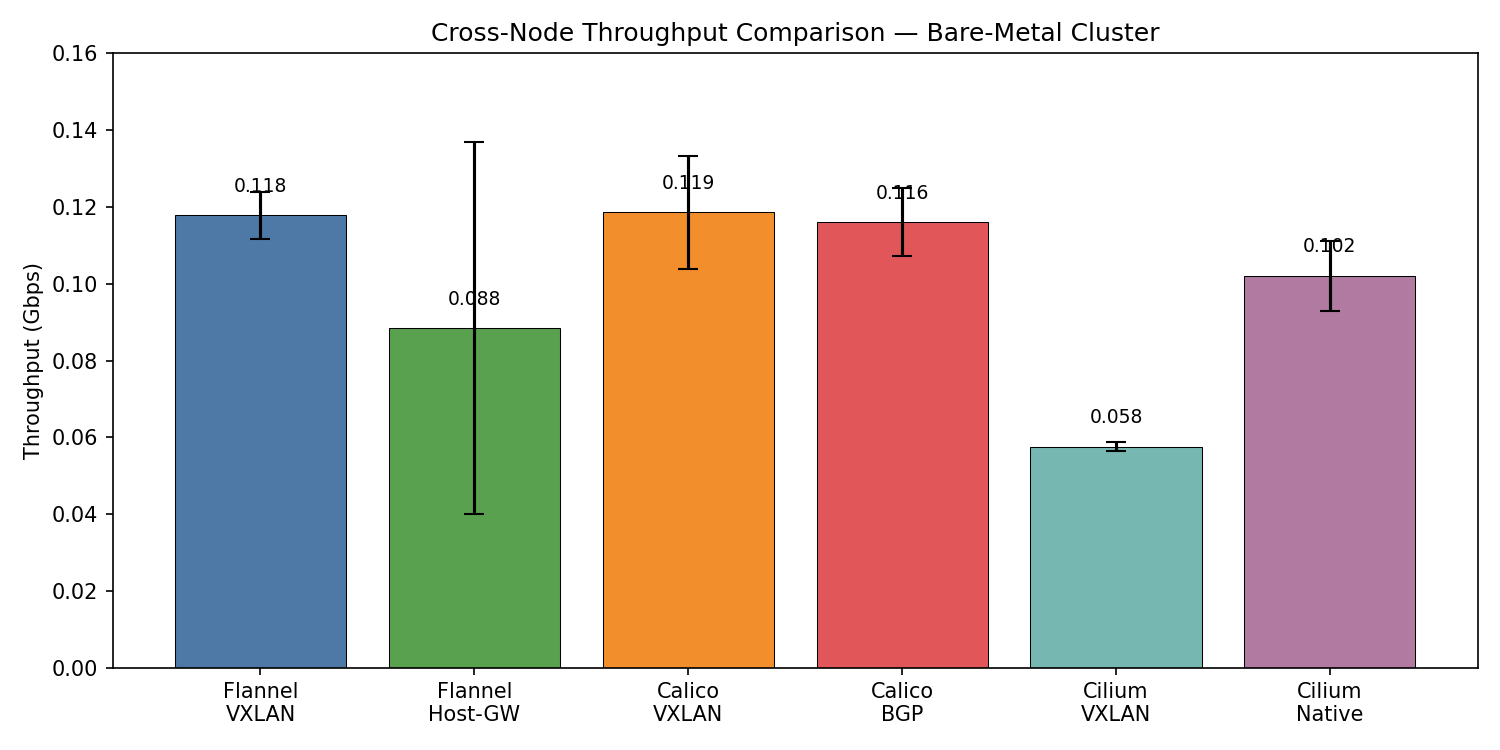
\includegraphics[width=\textwidth]{bare-metal/plots/1_throughput_comparison.png}
  \caption{Cross-node TCP throughput comparison across six CNI configurations. Error bars show standard deviation over 4--5 runs.}
  \label{fig:bm-throughput-fig}
\end{figure}

\begin{table}[H]
\centering
\caption{Cross-Node TCP Throughput (Gbps) --- Per-Run Values}
\small
\begin{tabular}{lrrrrrrr}
  \toprule
  \textbf{CNI Config} & \textbf{Run 1} & \textbf{Run 2} & \textbf{Run 3} & \textbf{Run 4} & \textbf{Run 5} & \textbf{Mean} & \textbf{Stdev} \\
  \midrule
  Flannel VXLAN  & 0.121 & 0.120 & 0.120 & 0.121 & 0.107 & 0.118 & 0.006 \\
  Flannel Host-GW & 0.034 & 0.036 & 0.119 & 0.125 & 0.127 & 0.088 & 0.049 \\
  Calico VXLAN   & 0.115 & 0.117 & 0.125 & 0.138 & 0.098 & 0.119 & 0.015 \\
  Calico BGP     & 0.126 & 0.119 & 0.114 & 0.105 & ---   & 0.116 & 0.009 \\
  Cilium VXLAN   & 0.058 & 0.058 & 0.057 & 0.056 & 0.059 & 0.058 & 0.001 \\
  Cilium Underlay  & 0.096 & 0.108 & 0.096 & 0.115 & 0.095 & 0.102 & 0.009 \\
  \bottomrule
\end{tabular}
\label{tab:bm-throughput}
\end{table}

\begin{findingbox}[Bare-Metal Throughput Key Observations]
\begin{enumerate}
  \item \textbf{Calico VXLAN and Flannel VXLAN lead}: Both overlay configurations achieve $\approx$0.118--0.119\,Gbps, suggesting that at WiFi bandwidth levels, VXLAN encapsulation overhead is negligible relative to the physical medium's throughput ceiling.
  \item \textbf{Cilium VXLAN is anomalously slow}: At 0.058\,Gbps---roughly half of other configurations---Cilium's eBPF VXLAN path has significant fixed overhead. Unlike Flannel's simple kernel VXLAN socket, Cilium attaches eBPF programs at the TC layer, processing every packet through eBPF maps for connection tracking and policy enforcement even with no NetworkPolicy applied. On WiFi, this per-packet eBPF invocation cost becomes dominant---making eBPF overhead \emph{link-speed dependent}.
  \item \textbf{Flannel Host-GW cold-start effect}: First two runs (0.034, 0.036\,Gbps) are $\approx$70\% slower than subsequent runs (0.119--0.127\,Gbps), reflecting ARP cache convergence on WiFi: the kernel must resolve MAC addresses via WiFi broadcast frames. Runs~3--5 reflect warm cache state. This warmup effect is absent in VXLAN modes, which maintain persistent tunnel endpoints.
  \item \textbf{Cilium VXLAN has lowest variance}: Stdev 0.001\,Gbps indicates deterministic (though slow) behavior.
\end{enumerate}
\end{findingbox}

\subsubsection{TCP\_RR Latency (netperf)}

\begin{figure}[H]
  \centering
  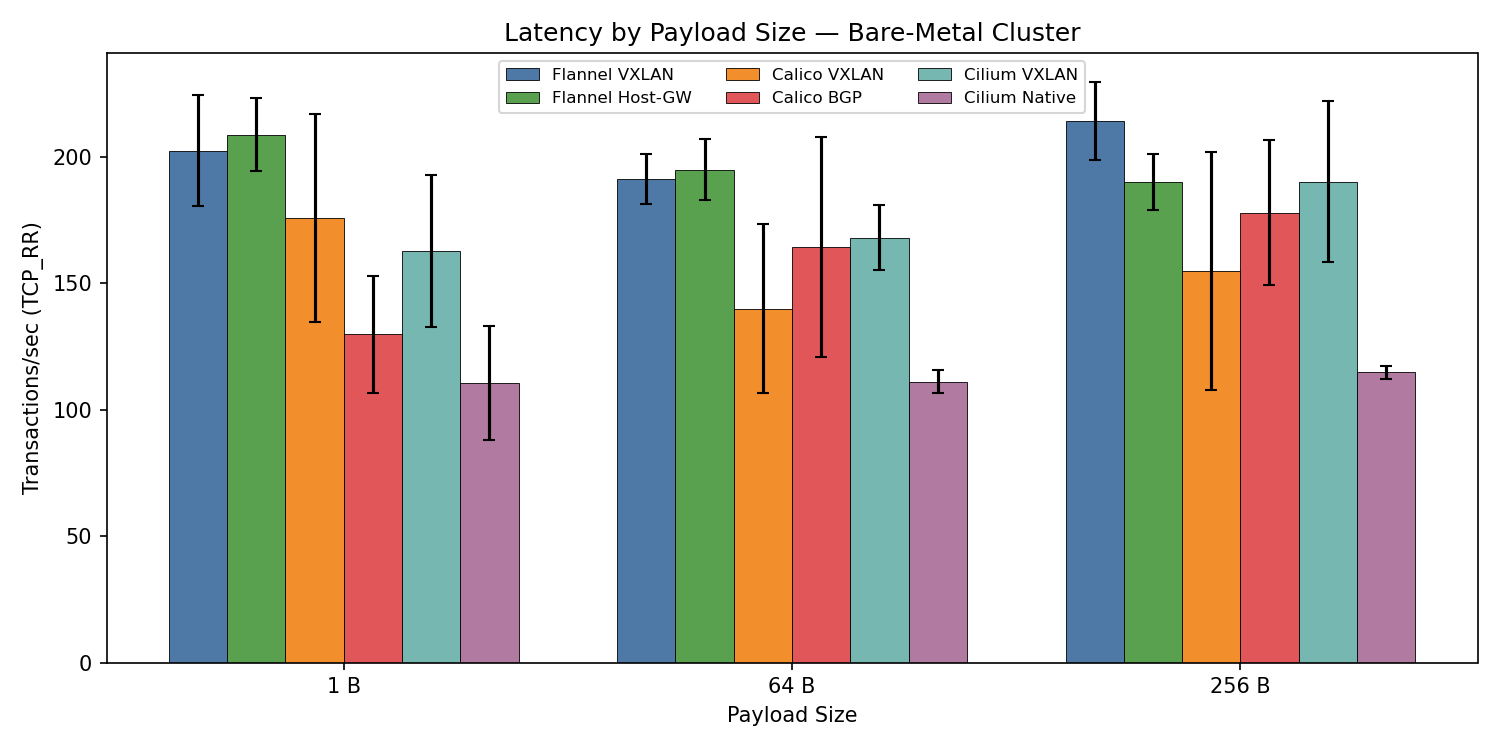
\includegraphics[width=\textwidth]{bare-metal/plots/1_latency_comparison.png}
  \caption{TCP\_RR transaction rate across six CNI configurations and three payload sizes.}
  \label{fig:bm-latency-fig}
\end{figure}

\begin{table}[H]
\centering
\caption{TCP\_RR Transaction Rate (trans/sec) --- Mean $\pm$ Stdev over 5 Runs}
\begin{tabular}{lrrrrrr}
  \toprule
  \multirow{2}{*}{\textbf{Payload}} & \multicolumn{2}{c}{\textbf{Flannel}} & \multicolumn{2}{c}{\textbf{Calico}} & \multicolumn{2}{c}{\textbf{Cilium}} \\
  \cmidrule(lr){2-3}\cmidrule(lr){4-5}\cmidrule(lr){6-7}
  & VXLAN & Host-GW & VXLAN & BGP & VXLAN & Underlay \\
  \midrule
  1\,B    & 202\,$\pm$\,22 & 209\,$\pm$\,15 & 176\,$\pm$\,41 & 130\,$\pm$\,23 & 163\,$\pm$\,30 & 111\,$\pm$\,23 \\
  64\,B   & 191\,$\pm$\,10 & 195\,$\pm$\,12 & 140\,$\pm$\,33 & 164\,$\pm$\,44 & 168\,$\pm$\,13 & 111\,$\pm$\,5 \\
  256\,B  & 214\,$\pm$\,15 & 190\,$\pm$\,11 & 155\,$\pm$\,47 & 178\,$\pm$\,29 & 190\,$\pm$\,32 & 115\,$\pm$\,3 \\
  \bottomrule
\end{tabular}
\label{tab:bm-latency}
\end{table}

\begin{findingbox}[Bare-Metal Latency Key Observations]
\begin{enumerate}
  \item \textbf{Flannel dominates TCP\_RR}: Both modes achieve the highest transaction rates (190--214\,trans/sec), reflecting lightweight per-packet processing.
  \item \textbf{Cilium Underlay is consistently slowest}: 111--115\,trans/sec with remarkably low variance (stdev 3--23). Underlay routing eBPF programs add more per-transaction overhead than the VXLAN fast-path.
  \item \textbf{Calico shows high variability}: Stdev 23--47\,trans/sec, likely from WiFi interference interacting with iptables processing.
\end{enumerate}
\end{findingbox}

\subsubsection{HTTP Performance (Fortio)}

\begin{figure}[H]
  \centering
  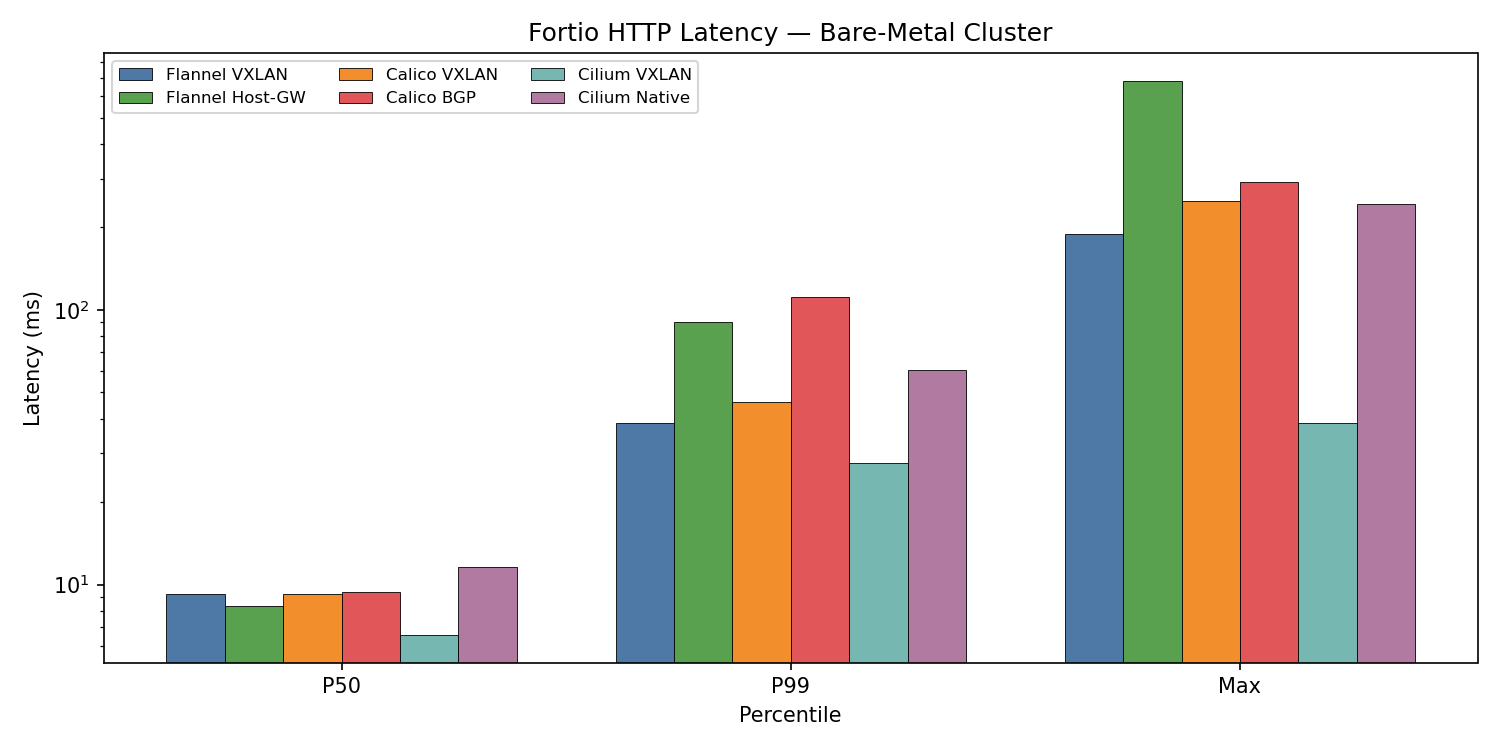
\includegraphics[width=\textwidth]{bare-metal/plots/1_fortio_comparison.png}
  \caption{Fortio HTTP latency percentiles across six CNI configurations.}
  \label{fig:bm-fortio-fig}
\end{figure}

\begin{table}[H]
\centering
\caption{Fortio HTTP Latency (ms) --- Mean over 4--5 Runs}
\begin{tabular}{lrrrrrr}
  \toprule
  \multirow{2}{*}{\textbf{Percentile}} & \multicolumn{2}{c}{\textbf{Flannel}} & \multicolumn{2}{c}{\textbf{Calico}} & \multicolumn{2}{c}{\textbf{Cilium}} \\
  \cmidrule(lr){2-3}\cmidrule(lr){4-5}\cmidrule(lr){6-7}
  & VXLAN & Host-GW & VXLAN & BGP & VXLAN & Underlay \\
  \midrule
  P50  & 9.26 & 8.34 & 9.23 & 9.36 & \textbf{6.56} & 11.54 \\
  P99  & 38.77 & 90.33 & 46.21 & 111.24 & \textbf{27.75} & 60.19 \\
  Max  & 188.54 & 681.78 & 248.93 & 291.04 & \textbf{38.72} & 242.44 \\
  \bottomrule
\end{tabular}
\label{tab:bm-fortio}
\end{table}

\begin{findingbox}[Bare-Metal HTTP Key Observations]
\begin{enumerate}
  \item \textbf{Cilium VXLAN achieves best HTTP latency}: P50\,=\,6.56\,ms, P99\,=\,27.75\,ms, Max\,=\,38.72\,ms. Despite lowest throughput, eBPF excels at request-response handling---$\approx$21\% lower P50 than next-best (Flannel Host-GW, 8.34\,ms).
  \item \textbf{Cilium VXLAN has lowest tail latency}: Max of 38.72\,ms vs.\ 188--682\,ms for others. eBPF's deterministic processing insulates against WiFi-induced spikes.
  \item \textbf{Flannel Host-GW shows severe tail latency}: P50 is second-best (8.34\,ms) but Max reaches 681.78\,ms, indicating vulnerability to WiFi ARP failures.
\end{enumerate}
\end{findingbox}

\subsubsection{UDP Performance (iperf3)}

\begin{table}[H]
\centering
\caption{UDP Performance --- Overall Averages per CNI (9 runs: 3 targets $\times$ 3 repetitions)}
\small
\begin{tabular}{lrrrrrr}
  \toprule
  \textbf{CNI Config} & \textbf{Tput (Mbps)} & \textbf{$\pm$Stdev} & \textbf{Loss (\%)} & \textbf{$\pm$Stdev} & \textbf{Jitter (ms)} & \textbf{$\pm$Stdev} \\
  \midrule
  Calico BGP        & \textbf{11.88} & 2.86 & \textbf{38.15} & 31.28 & 1.81 & 1.47 \\
  Cilium Underlay     & 10.36 & 1.07 & 42.37 & 33.23 & \textbf{1.47} & 0.35 \\
  Flannel VXLAN     & 9.98  & 1.81 & 46.50 & 31.61 & 1.94 & 1.62 \\
  Flannel Host-GW   & 8.67  & 3.05 & 57.94 & 23.40 & 3.36 & 2.36 \\
  Cilium VXLAN      & 7.94  & 3.10 & 38.02 & 34.59 & 1.55 & 1.04 \\
  Calico VXLAN      & 5.78  & 3.44 & 68.33 & 26.43 & 13.34 & 16.11 \\
  \bottomrule
\end{tabular}
\label{tab:bm-udp}
\end{table}

\begin{table}[H]
\centering
\caption{UDP Throughput (Mbps) and Loss (\%) by Bandwidth Target (3-run means)}
\small
\resizebox{\textwidth}{!}{%
\begin{tabular}{l rr rr rr}
  \toprule
  & \multicolumn{2}{c}{\textbf{10\,Mbps}} & \multicolumn{2}{c}{\textbf{25\,Mbps}} & \multicolumn{2}{c}{\textbf{50\,Mbps}} \\
  \cmidrule(lr){2-3}\cmidrule(lr){4-5}\cmidrule(lr){6-7}
  \textbf{CNI Config} & Tput & Loss & Tput & Loss & Tput & Loss \\
  \midrule
  Calico BGP      & 9.97  & 0.11  & 12.37 & 44.67 & 13.29 & 69.67 \\
  Cilium Underlay   & 9.52  & 0.12  & 10.23 & 52.33 & 11.33 & 74.67 \\
  Flannel VXLAN   & 9.11  & 6.83  & 10.27 & 57.00 & 10.58 & 75.67 \\
  Flannel Host-GW & 6.18  & 34.83 & 9.11  & 61.33 & 10.72 & 77.67 \\
  Cilium VXLAN    & 8.68  & 4.71  & 9.53  & 55.00 & 5.60  & 54.33 \\
  Calico VXLAN    & 5.00  & 43.00 & 4.34  & 80.00 & 7.99  & 82.00 \\
  \bottomrule
\end{tabular}%
}
\label{tab:bm-udp-bw}
\end{table}

\begin{findingbox}[Bare-Metal UDP Key Observations]
\begin{enumerate}
  \item \textbf{Calico BGP leads UDP}: 11.88\,Mbps throughput, 38\% loss. At 10\,Mbps, near-perfect delivery (0.11\% loss).
  \item \textbf{Calico VXLAN suffers severe degradation}: 5.78\,Mbps with 68\% loss and extreme jitter (13.34\,ms $\pm$ 16.11). VXLAN + iptables creates a bottleneck for connectionless UDP.
  \item \textbf{Calico BGP and Cilium Underlay excel at UDP}: Both achieve near-zero loss at 10\,Mbps (0.11\% and 0.12\%). However, Flannel Host-GW (also underlay) suffers 34.83\% loss, indicating underlay routing alone does not guarantee better UDP---the CNI's architecture matters more.
  \item \textbf{Cilium Underlay has lowest jitter}: 1.47\,ms $\pm$ 0.35, consistent with its low-variance TCP\_RR behavior.
  \item \textbf{Loss scales with bandwidth target}: $<$7\% at 10\,Mbps (except Calico VXLAN and Flannel Host-GW) but 54--82\% at 50\,Mbps.
\end{enumerate}
\end{findingbox}

\subsubsection{CPU Overhead}



\begin{table}[H]
\centering
\caption{CPU During Fortio (avg across all sampled pods)}
\begin{tabular}{lrll}
  \toprule
  \textbf{CNI Config} & \textbf{Avg (mcpu)} &  \\
  \midrule
  Cilium Underlay   & 6.8  & \\
  Calico BGP      & 8.2  & \\
  Flannel Host-GW & 8.3  &  \\
  Flannel VXLAN   & 8.4  &  \\
  Cilium VXLAN    & 10.2 & \\
  Calico VXLAN    & 14.7\textsuperscript{\dag} & \\
  \bottomrule
\end{tabular}
\label{tab:bm-cpu-pods}
\end{table}



\begin{findingbox}[Bare-Metal CPU Key Observations]
\begin{enumerate}
  \item \textbf{All CNIs have modest CPU overhead}: 3.9--6.0\% node-level. At WiFi-constrained packet rates ($\approx$10,000\,pps), no CNI's datapath processing approaches CPU saturation.
  \item \textbf{Flannel VXLAN is lightest}: 3.9\% average---consistent with its minimal per-packet processing design.
  \item \textbf{Calico BGP has highest node CPU}: 6.0\%, with BGP daemon and contributing 12--34\,m per calico-node pod.
\end{enumerate}
\end{findingbox}

\subsubsection{Overlay vs.\ Underlay Routing Comparison}

\begin{figure}[H]
  \centering
  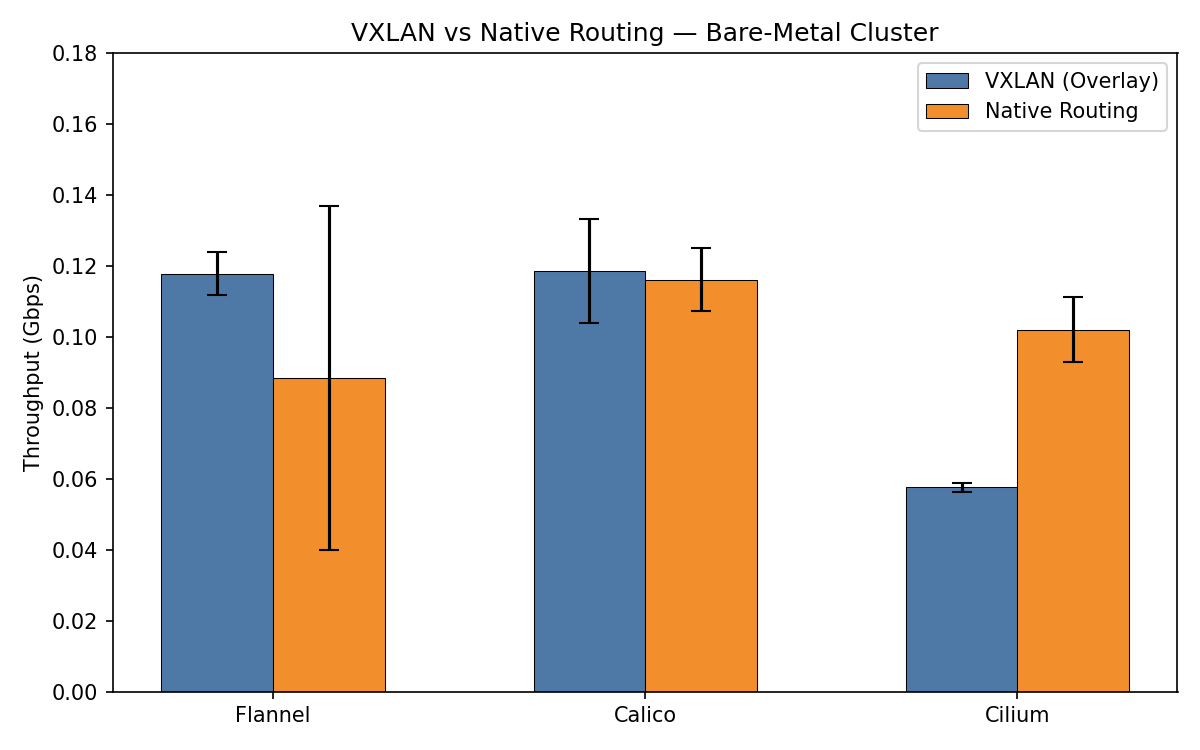
\includegraphics[width=0.85\textwidth]{bare-metal/plots/1_encapsulation_comparison.png}
  \caption{VXLAN overlay vs.\ underlay routing throughput for each CNI.}
  \label{fig:bm-encap-fig}
\end{figure}

\begin{table}[H]
\centering
\caption{VXLAN vs.\ Underlay Routing --- Summary}
\begin{tabular}{lrrrl}
  \toprule
  \textbf{CNI} & \textbf{VXLAN (Gbps)} & \textbf{Underlay (Gbps)} & \textbf{$\Delta$} & \textbf{Winner} \\
  \midrule
  Flannel & 0.118 & 0.088\textsuperscript{\dag} & $-25\%$ & VXLAN \\
  Calico  & 0.119 & 0.116 & $-2\%$ & $\approx$ tie \\
  Cilium  & 0.058 & 0.102 & $+77\%$ & Underlay \\
  \bottomrule
\end{tabular}
\label{tab:bm-encap}
\end{table}

{\footnotesize \textsuperscript{\dag}Flannel Host-GW mean includes two cold-start runs. Excluding these, stable-state mean is 0.124\,Gbps ($+5\%$ over VXLAN).}

\begin{findingbox}[Overlay vs.\ Underlay: Analysis]
The comparison yields a CNI-specific picture, not a universal verdict:

\paragraph{Flannel:} VXLAN outperforms Host-GW on mean throughput due to Host-GW's warmup penalty. Once warmed, Host-GW achieves 0.124\,Gbps vs.\ VXLAN's 0.118\,Gbps. However, Host-GW's Fortio Max (681.78\,ms) reveals vulnerability to WiFi ARP failures.

\paragraph{Calico:} Essentially identical---VXLAN (0.119) vs.\ BGP (0.116\,Gbps, $-2\%$). At WiFi throughput levels, VXLAN's 50-byte overhead is dwarfed by the wireless medium's latency.

\paragraph{Cilium:} The only CNI where mode matters dramatically. Underlay (0.102\,Gbps) delivers 77\% higher throughput than VXLAN (0.058\,Gbps). Cilium's eBPF VXLAN path has substantial per-packet overhead. Interestingly, VXLAN achieves much better HTTP latency (P50: 6.56 vs.\ 11.54\,ms), indicating the VXLAN eBPF fast-path is optimized for request-level processing.
\end{findingbox}



\subsection{Bare-Metal Analysis and Discussion}

\subsubsection{The ``Edge Environment'' Paradox}

While industry benchmarks often favor Cilium and Calico for large-scale datacenters, our 3-node WiFi cluster results demonstrate that \textbf{simplicity outperforms sophistication} in resource-constrained or high-latency environments:

\begin{itemize}
  \item \textbf{Flannel wins on latency:} Its ``passive'' architecture---simply wrapping packets and handing them to the kernel without deep packet inspection---leaves more CPU headroom for the OS to manage WiFi signal jitter and retransmissions.
  \item \textbf{Cilium Underlay performance penalty:} Cilium Underlay (111\,trans/sec) is slower than its own VXLAN path in TCP\_RR because the underlay eBPF programs execute complex security identity checks on every packet. On WiFi, this ``intelligence'' is slower than simple encapsulation.
  \item \textbf{Calico's management tax:} 6.0\% CPU reflects BGP daemon (BIRD) and Felix agent overhead---unnecessary for a 3-node cluster where BGP's scalability benefits cannot manifest.
\end{itemize}

\subsubsection{Throughput--Latency Inversion in Cilium VXLAN}

Cilium VXLAN has the \emph{worst} TCP throughput (0.058\,Gbps) but the \emph{best} HTTP P50/P99/Max latency (6.56/27.75/38.72\,ms). This apparent contradiction reveals a fundamental architectural distinction:

\begin{itemize}
  \item \textbf{TCP throughput} measures sustained bandwidth where per-packet eBPF overhead accumulates multiplicatively, halving effective bulk throughput on WiFi.
  \item \textbf{HTTP latency} measures individual request-response cycles where eBPF's O(1) connection tracking lookup and iptables bypass provide a per-request advantage regardless of link speed.
\end{itemize}

\noindent\textbf{Practical implication:} Microservice workloads on constrained networks should prefer Cilium VXLAN despite its bandwidth penalty---the P99 advantage (27.75\,ms vs.\ 38--111\,ms) is critical for SLA compliance.

\subsubsection{UDP Comparison Caveat}

While UDP results provide useful relative rankings, direct cross-CNI comparison is limited by high packet loss (38--68\% overall). At 10\,Mbps---the only rate where WiFi is not saturated---only Calico BGP and Cilium Underlay achieve near-perfect delivery ($<$0.15\% loss). The 25--50\,Mbps targets drive all CNIs past WiFi capacity, making these rates a measure of saturation behavior rather than CNI differentiation.

\subsubsection{CPU Overhead: Deeper Interpretation}

At 0.119\,Gbps with 1500-byte MTU, nodes process approximately 10,000 packets/second---well below the millions/second threshold where eBPF vs.\ iptables differences manifest. This explains the uniformly modest CPU usage (3.9--6.0\%). The Calico VXLAN kube-apiserver spike (135.5\,mcpu) likely reflects Felix daemon polling rather than data-plane overhead, highlighting that \textbf{Calico's control plane is tightly coupled to the apiserver}.


% ========================================================================
% CROSS-ENVIRONMENT ANALYSIS
% ========================================================================
\newpage
\section{Cross-Environment Comparative Analysis}

This section compares findings across the kind-cluster (intra-node, Docker bridge) and bare-metal (multi-node WiFi) environments to identify which properties are environment-dependent and which are intrinsic to the CNI architectures.

\subsection{Throughput Comparison}

\begin{table}[H]
\centering
\caption{Kind Cluster vs.\ Bare-Metal --- Throughput Comparison}
\begin{tabular}{lrrr}
  \toprule
  \textbf{CNI} & \textbf{Kind T2 (Gbps)} & \textbf{Bare-Metal (Gbps)} & \textbf{Ratio} \\
  \midrule
  Flannel VXLAN & 30.96 & 0.118 & 262$\times$ \\
  Calico VXLAN  & 23.83 & 0.119 & 200$\times$ \\
  Cilium VXLAN  & 27.40 & 0.058 & 472$\times$ \\
  \bottomrule
\end{tabular}
\label{tab:cross-throughput}
\end{table}

{\footnotesize Kind-cluster values: T2 cross-node, 1\,MB, $c=16$ (representative middle-ground configuration).}

The 200--472$\times$ throughput gap confirms that Docker's virtual bridge is far more efficient than physical WiFi. Cilium's ratio (472$\times$) is much larger than Flannel's (262$\times$), indicating that Cilium's eBPF VXLAN overhead is amplified on constrained physical networks. In kind-cluster, the 128-core server provides enough CPU headroom to mask per-packet processing costs; on WiFi, each packet's overhead becomes proportionally significant.

\subsection{Ranking Inversions}

\begin{table}[H]
\centering
\caption{CNI Ranking Shifts Between Environments}
\begin{tabular}{lll}
  \toprule
  \textbf{Metric} & \textbf{Kind-Cluster Ranking} & \textbf{Bare-Metal Ranking} \\
  \midrule
  TCP Throughput & Cilium $>$ Flannel $>$ Calico & Calico VXLAN $\approx$ Flannel $>$ Cilium \\
  Latency & Flannel $\approx$ Cilium $>$ Calico & Flannel $>$ Cilium VXLAN $>$ Calico \\
  HTTP Perf & Cilium $>$ Flannel $\approx$ Calico & Cilium VXLAN $>$ Flannel $>$ Calico \\
  \bottomrule
\end{tabular}
\label{tab:ranking-shifts}
\end{table}

\begin{findingbox}[Key Cross-Environment Insights]
\begin{enumerate}
  \item \textbf{Cilium's throughput ranking inverts}: Leads in kind-cluster (63.98\,Gbps same-node) but trails in bare-metal WiFi (0.058\,Gbps VXLAN). The eBPF fast-path advantage requires sufficient link bandwidth to manifest; on a slow link, per-packet overhead dominates.

  \item \textbf{Cilium VXLAN's HTTP advantage is consistent}: Best HTTP latency in both environments. In kind-cluster: highest Fortio QPS at 64\,B/$c{=}16$ (132,836 vs.\ 81,749 for Flannel). In bare-metal: best P50 (6.56\,ms), P99 (27.75\,ms), and Max (38.72\,ms). eBPF's efficient request-response handling is an \emph{intrinsic} CNI property that transfers across environments.

  \item \textbf{Flannel's low latency is consistent}: Delivers the lowest TCP\_RR latency in both environments (24.18\,$\mu$s in kind, 190--214\,trans/sec in bare-metal). Its lightweight architecture is universally beneficial.

  \item \textbf{Calico's iptables overhead is universal}: Calico trails other CNIs in both environments for raw throughput and latency. The iptables rule traversal cost is a consistent architectural penalty.

  \item \textbf{Environment amplifies architectural differences}: The kind-cluster's Docker bridge masks many CNI processing differences (all CNIs are fast when the ``network'' is memory copy). Physical WiFi amplifies these differences by making every packet's processing overhead matter.

  \item \textbf{Overlay vs.\ underlay is environment-dependent}: In kind-cluster (Docker bridge), VXLAN encapsulation adds minimal overhead. In bare-metal, Cilium Underlay outperforms Cilium VXLAN by 77\% for throughput, while Flannel and Calico show negligible differences between modes.
\end{enumerate}
\end{findingbox}

\subsection{Latency Scale Analysis}

\begin{table}[H]
\centering
\caption{TCP\_RR Latency Scale Comparison}
\begin{tabular}{lrrl}
  \toprule
  \textbf{CNI} & \textbf{Kind ($\mu$s)} & \textbf{Bare-Metal ($\mu$s)} & \textbf{Scaling Factor} \\
  \midrule
  Flannel VXLAN & 24.18 & $\approx$4{,}950\textsuperscript{a} & 205$\times$ \\
  Calico VXLAN  & 32.91 & $\approx$7{,}140\textsuperscript{a} & 217$\times$ \\
  Cilium VXLAN  & 24.63 & $\approx$5{,}950\textsuperscript{a} & 242$\times$ \\
  \bottomrule
\end{tabular}
\label{tab:cross-latency}
\end{table}

{\footnotesize \textsuperscript{a}Bare-metal latency estimated from 64\,B TCP\_RR trans/sec: $1{,}000{,}000 / \text{trans\_per\_sec}$.}

\noindent The 200--242$\times$ latency scaling confirms that WiFi RTT ($\approx$5--10\,ms) dominates over software processing differences ($\approx$25--33\,$\mu$s in kind). Cilium's larger scaling factor (242$\times$) vs.\ Flannel (205$\times$) is consistent with the throughput analysis: Cilium's per-packet overhead is amplified more by constrained networks.

\subsection{Environment-Conditioned Interpretation}

These results should be interpreted as \textbf{environment-conditioned findings} rather than universal CNI rankings:

\begin{itemize}
  \item The kind-cluster measures \textbf{CNI software efficiency} in isolation, where the ``network'' is essentially memory copy between Docker containers. Rankings here reflect CPU processing overhead.
  \item The bare-metal WiFi cluster measures \textbf{CNI behavior under physical network constraints}, where the wireless medium dominates and compresses all CNIs into a narrow performance band. Rankings here reflect how well each CNI handles a slow, variable link.
  \item Production environments (wired 1--100\,GbE) would likely produce intermediate results, with CNI processing overhead becoming visible but not as amplified as on WiFi.
\end{itemize}


% ======================== RELATED WORK ========================
\section{Related Work}

\begin{itemize}
  \item \textbf{Qi et al.\ (2021)} benchmarked CNI plugins in bare-metal and AWS environments, finding Calico BGP fastest in bare-metal. Our bare-metal results partially confirm this, but show that physical medium can dominate CNI differences.
  \item \textbf{Kubernetes network benchmark project (CNCF 2019)} provided automated frameworks but lacked extension comparisons and cross-environment analysis.
  \item \textbf{Cilium documentation} provides internal benchmarks showing eBPF advantages. We confirm these for kind-cluster but find them inverted on constrained WiFi networks.
  \item This study extends prior work by: (a) systematically comparing overlay vs.\ underlay routing for all three CNIs on the same hardware, (b) evaluating NetworkPolicy, WireGuard, and KPR overhead, and (c) providing direct cross-environment comparison between simulated and physical deployments.
\end{itemize}

% ======================== OUTCOMES AND CONCLUSION ========================
\section{Outcomes and Conclusion}

This study presents a comprehensive performance comparison of Flannel, Calico, and Cilium CNI plugins across two environments: a kind-cluster (729 baseline tests + 3 extensions) and a bare-metal WiFi cluster (90+ benchmark runs across 6 configurations + UDP + CPU monitoring). Key findings:

\begin{enumerate}
  \item \textbf{Cilium leads throughput in kind-cluster}: Up to 63.98\,Gbps same-node via eBPF fast-path. But this advantage does not transfer to bare-metal WiFi, where Cilium VXLAN trails at 0.058\,Gbps.

  \item \textbf{Flannel consistently delivers lowest latency}: 24.18\,$\mu$s in kind-cluster (64\,B TCP\_RR), 190--214\,trans/sec in bare-metal. Its minimalist architecture provides universally low overhead.

  \item \textbf{Cilium VXLAN's HTTP superiority is intrinsic}: Best HTTP latency in both environments (kind: highest Fortio QPS; bare-metal: P50\,=\,6.56\,ms, Max\,=\,38.72\,ms). eBPF's efficient request-response handling transfers across any physical medium.

  \item \textbf{WireGuard encryption is expensive}: $+537\%$ latency for Calico, $+365\%$ for Cilium. Cilium's eBPF integration mitigates some overhead. Deploy with careful capacity planning.

  \item \textbf{NetworkPolicy impact is implementation-dependent}: $-45\%$ throughput for Calico (iptables), $+118\%$ for Cilium (eBPF; high CV). Latency impact negligible for both.

  \item \textbf{Overlay vs.\ underlay routing is CNI-specific}: Flannel Host-GW $\geq$ VXLAN (once warm), Calico VXLAN $\approx$ BGP, Cilium Underlay $\gg$ VXLAN ($+77\%$). No universal winner.

  \item \textbf{Calico BGP dominates UDP on bare-metal}: 11.88\,Mbps, 38\% loss. Calico VXLAN is worst (5.78\,Mbps, 68\% loss). Underlay routing eliminates per-packet encapsulation overhead for connectionless traffic.

  \item \textbf{CPU overhead is uniformly modest on bare-metal}: 3.9--6.0\% node-level, confirming WiFi---not CPU---is the bottleneck on constrained networks.

  \item \textbf{CNI rankings shift with hardware}: Production CNI selection must be validated on representative hardware, not extrapolated from simulated environments.
\end{enumerate}

\subsection{Recommendations}

\begin{resultbox}[CNI Selection Guidelines]
\begin{itemize}
  \item \textbf{Simple workloads, low-bandwidth networks:} Flannel---minimal overhead, lowest latency, lightest CPU (3.9\%), simplest operations.
  \item \textbf{Latency-sensitive microservices:} Cilium VXLAN---best HTTP P50/P99/Max across both environments. eBPF efficiently handles request-response workloads.
  \item \textbf{High-throughput environments (wired):} Cilium Underlay or Calico---Cilium leads in kind-cluster, Cilium Underlay offers $+77\%$ over VXLAN on bare-metal.
  \item \textbf{UDP-heavy workloads:} Calico BGP---highest UDP throughput, lowest loss at moderate rates.
  \item \textbf{Security requirements:} Calico for NetworkPolicy with proven iptables enforcement; Cilium for encryption (lower WireGuard overhead) and advanced observability (Hubble).
  \item \textbf{Large clusters with complex iptables:} Cilium KPR---bypass iptables entirely. Benefits scale with rule complexity.
\end{itemize}
\end{resultbox}

\begin{table}[H]
\centering
\caption{CNI Decision Matrix --- Quick Reference}
\begin{tabular}{p{3.8cm}p{3cm}p{6cm}}
  \toprule
  \textbf{Use Case} & \textbf{Recommended} & \textbf{Rationale} \\
  \midrule
  Constrained/WiFi network & Flannel VXLAN & Lowest CPU (3.9\%), consistent throughput \\
  Latency-critical services & Cilium VXLAN & Best P99 (27.75\,ms), lowest Max (38.72\,ms) \\
  High throughput (wired) & Cilium Underlay & +77\% over VXLAN on bare-metal \\
  UDP-heavy workloads & Calico BGP & Best UDP throughput, $<$0.15\% loss at 10\,Mbps \\
  Security-critical & Cilium & Lower WireGuard overhead ($+365\%$ vs.\ $+537\%$ Calico) \\
  Large clusters & Cilium KPR & Bypasses iptables rule explosion at scale \\
  Lowest complexity & Flannel VXLAN & No BGP/eBPF, minimal control plane \\
  \bottomrule
\end{tabular}
\label{tab:decision-matrix}
\end{table}

\subsection{Limitations}

\begin{itemize}
  \item \textbf{Kind environment:} All Part~A tests run inside Docker on a single host. Cross-node traffic traverses Docker's virtual bridge, not physical switches.
  \item \textbf{WiFi medium (Part~B):} The shared wireless link limits throughput to $\approx$0.12\,Gbps and introduces variance. Wired tests would better differentiate CNI processing overhead. However, the WiFi environment is also a deliberate research contribution: prior CNI benchmarks exclusively use wired Ethernet, leaving edge computing and development environment conditions uncharacterized.
  \item \textbf{VXLAN-only in kind:} Part~A tests VXLAN for all CNIs. BGP and underlay routing are only tested in Part~B.
  \item \textbf{No extension experiments on bare-metal:} NetworkPolicy, WireGuard, and KPR are only tested in kind-cluster.
  \item \textbf{Calico BGP with 4 runs (bare-metal):} One TCP throughput run failed, slightly reducing statistical confidence.
  \item \textbf{Cilium VXLAN UDP anomaly:} One run at 50\,Mbps recorded 0.00\,Mbps throughput (likely stalled).
  \item \textbf{CPU sampling:} \texttt{kubectl top} (bare-metal) provides 2\,s averages; \texttt{docker stats} (kind) samples every $\approx$3\,s. Both may miss sub-second spikes.
\end{itemize}

\subsection{Future Work}

\begin{itemize}
  \item Repeat benchmarks on wired Ethernet (1\,GbE, 10\,GbE) for intermediate comparison point
  \item Add extension experiments (NetworkPolicy, WireGuard, KPR) on bare-metal
  \item Test BGP mode for Calico in kind-cluster for overlay-vs-underlay comparison in both environments
  \item Profile per-packet CPU cost using perf/eBPF tracing
  \item Deploy application-level benchmarks (Redis, NGINX, gRPC)
  \item Evaluate Cilium Hubble observability overhead
\end{itemize}

% ======================== REFERENCES ========================
\section*{References}

\begin{enumerate}[label={[\arabic*]}]
  \item Flannel Project. ``flannel---Network fabric for containers.'' \url{https://github.com/flannel-io/flannel}
  \item Project Calico. ``Calico Networking for Kubernetes.'' \url{https://docs.tigera.io/calico/latest/about}
  \item Cilium Project. ``Cilium---eBPF-based Networking, Security, and Observability.'' \url{https://cilium.io/}
  \item kind Project. ``kind---Kubernetes IN Docker.'' \url{https://kind.sigs.k8s.io/}
  \item iperf3. ``A TCP, UDP, and SCTP network bandwidth measurement tool.'' \url{https://iperf.fr/}
  \item Netperf. ``Network Performance Benchmark.'' \url{https://hewlettpackard.github.io/netperf/}
  \item Fortio. ``Load testing library, command line tool, and web UI.'' \url{https://fortio.org/}
  \item WireGuard. ``Fast, Modern, Secure VPN Tunnel.'' \url{https://www.wireguard.com/}
  \item Qi, S.\ et~al.\ (2021). ``Assessing Container Network Interface Plugins: Functionality, Performance, and Scalability.'' \textit{IEEE Transactions on Network and Service Management}, 18(1).
  \item Kubernetes Documentation. ``Cluster Networking.'' \url{https://kubernetes.io/docs/concepts/cluster-administration/networking/}
  \item VXLAN RFC 7348. ``Virtual eXtensible Local Area Network.'' \url{https://datatracker.ietf.org/doc/html/rfc7348}
\end{enumerate}

\end{document}
